\chapter{Desarrollo del TFG}
\label{ch:desarrollo}

Este capítulo describe la metodología de trabajo empleada, la planificación en fases del proyecto y la ejecución detallada de los experimentos realizados para desarrollar y validar el sistema de detección de anomalías basado en Vision Transformers. Se documenta el proceso iterativo de optimización que condujo a la configuración final del modelo, así como los resultados obtenidos en cada fase experimental.

La Figura~\ref{fig:diagrama-fases-desarrollo} ofrece una visión global del flujo de trabajo seguido a lo largo del capítulo, permitiendo al lector situar cada sección en su contexto antes de entrar en el detalle. A efectos de seguimiento, se adopta la siguiente nomenclatura: (i) \textit{Preparación del conjunto de datos} designa el trabajo previo de curación y normalización de datos, articulado en cinco etapas (Etapas 1--5, con subetapas 4.1--4.4 donde corresponde); (ii) las Fases experimentales 1--4 corresponden a la experimentación propiamente dicha, con Experimentos en las Fases 1 y 3, e Iteraciones en la Fase 2. Esta distinción entre preparación y experimentación permite al lector localizar con precisión cada apartado del desarrollo.

\begin{figure}[htbp]
\centering
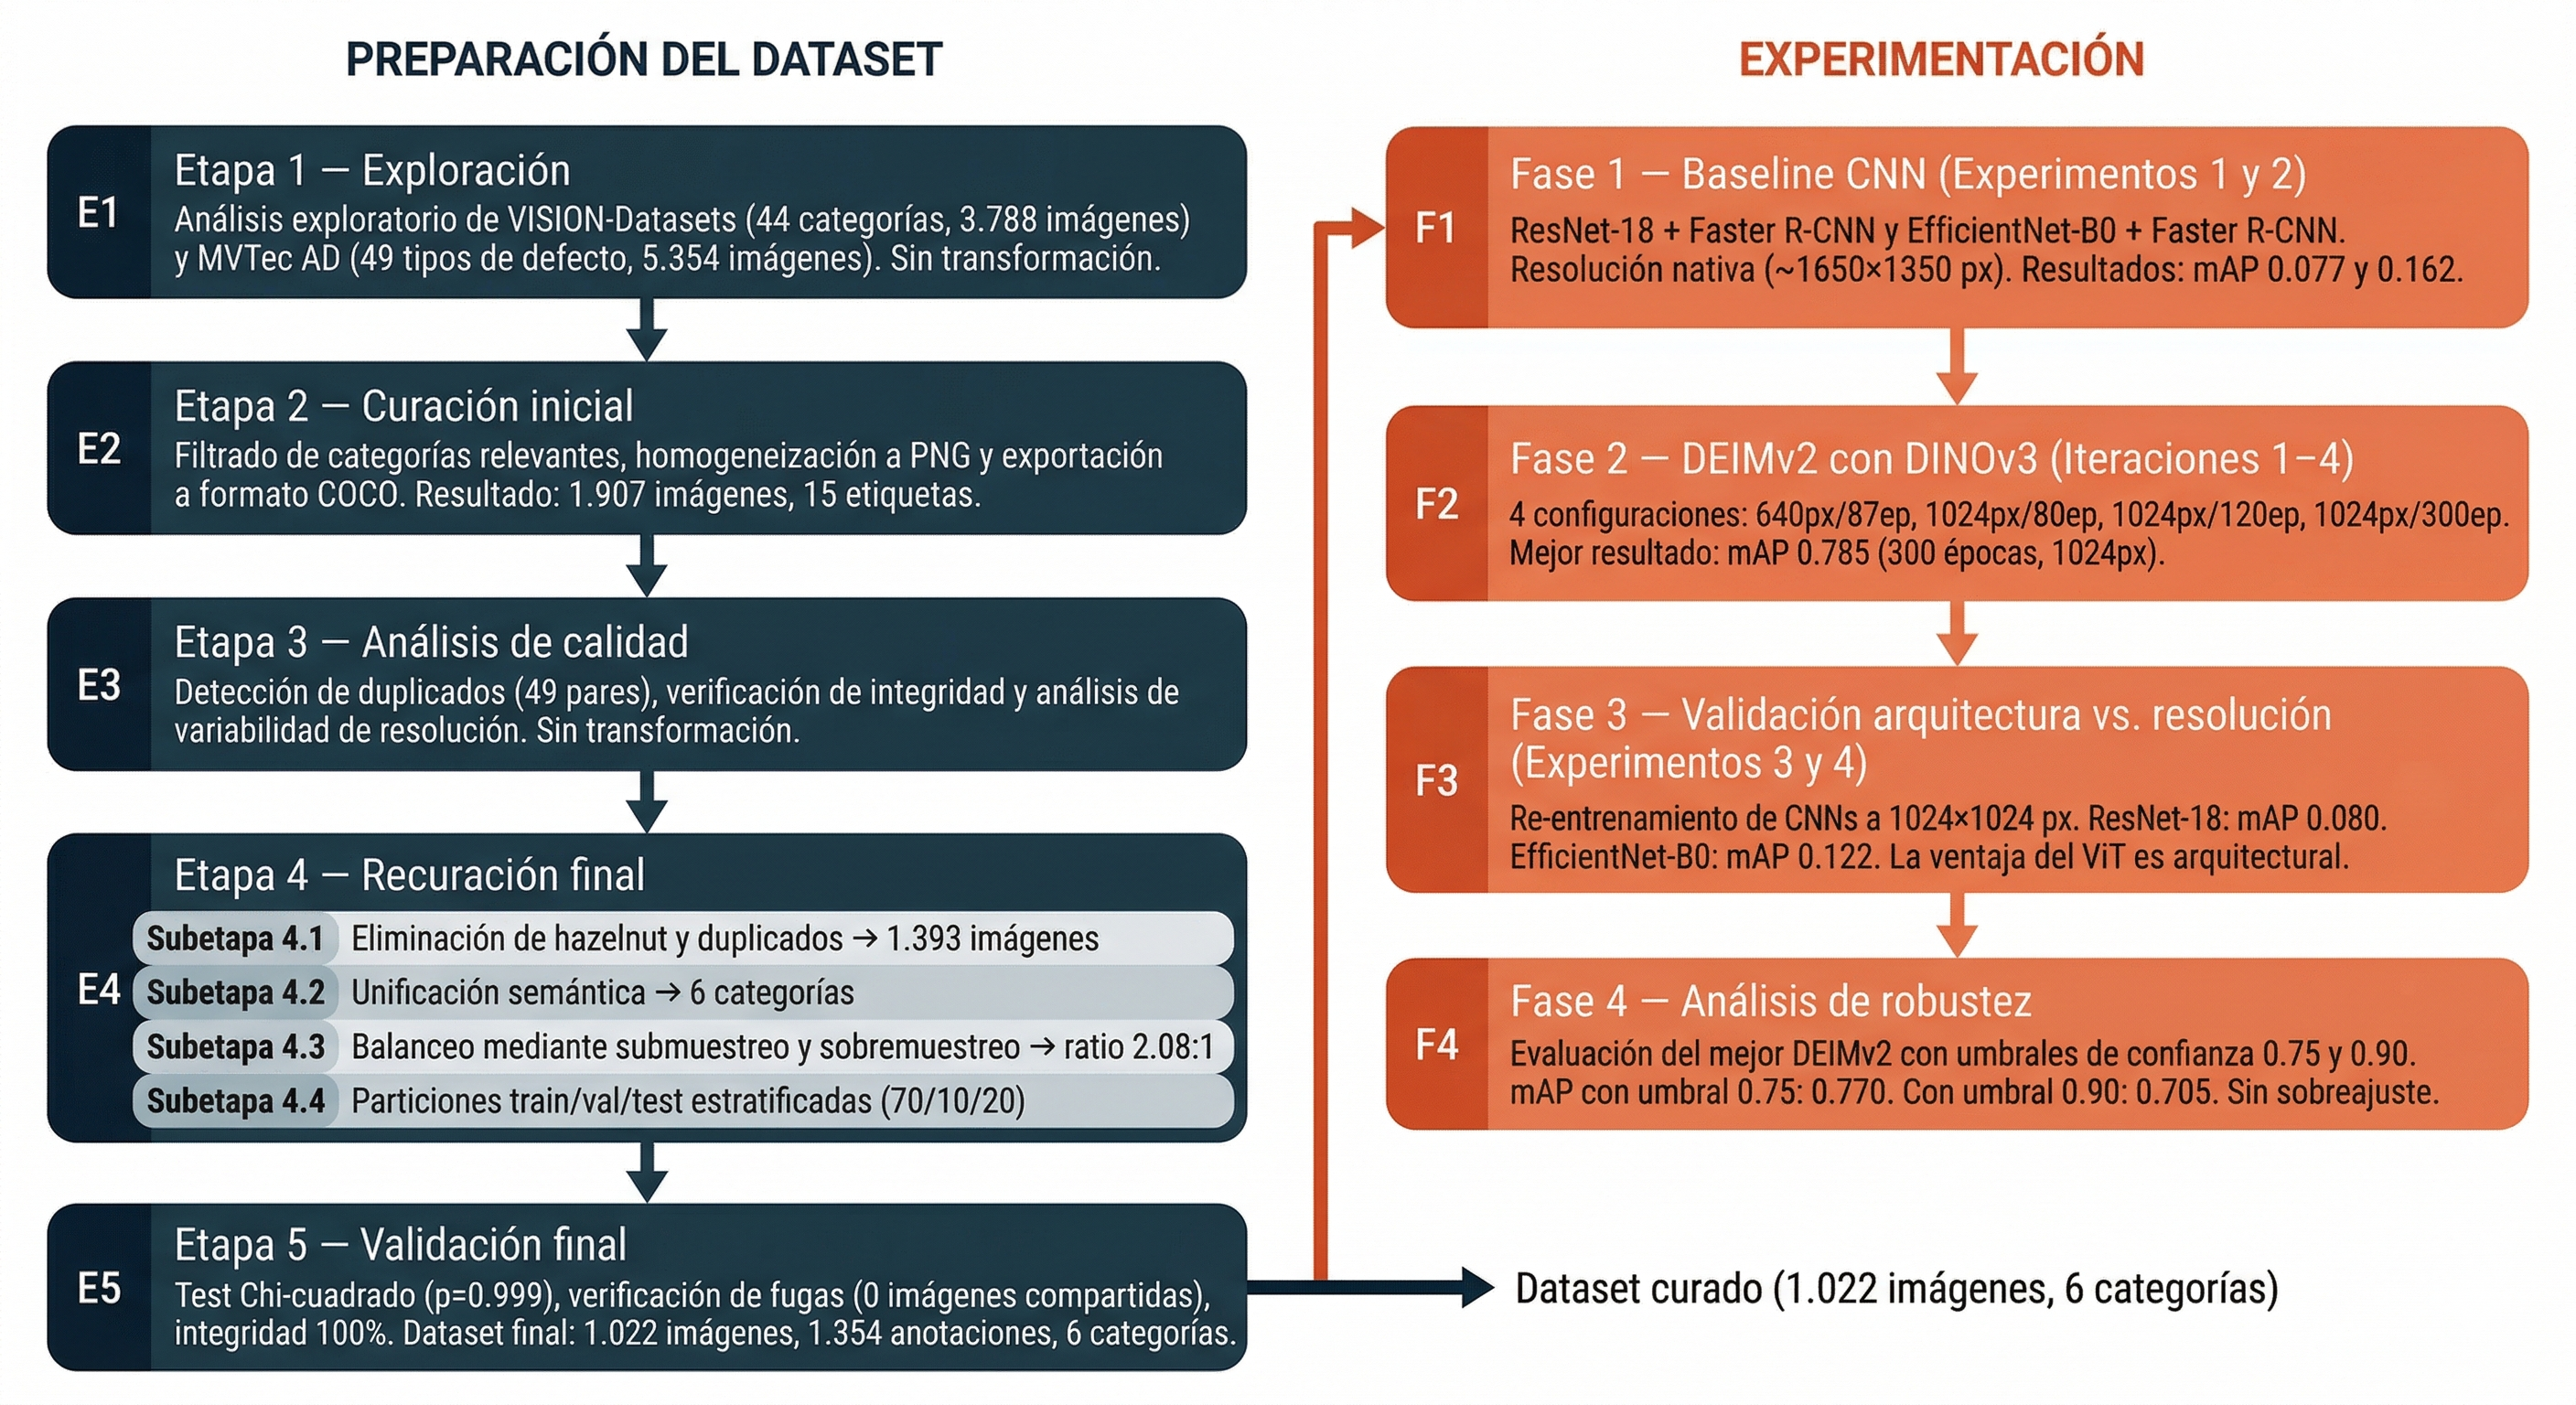
\includegraphics[width=1.0\textwidth]{fig/Diagrama-inicial-section-desarrollo.png}
\caption{Visión global del flujo de trabajo del Capítulo~\ref{ch:desarrollo}. El carril izquierdo recoge el bloque de \textit{Preparación del conjunto de datos} (Etapas E1--E5, con subetapas en la Etapa 4); el carril derecho corresponde al bloque de \textit{Experimentación} (Fases F1--F4). La flecha central indica que todas las fases experimentales consumen el conjunto de datos curado resultante de la Etapa 5 (1.022 imágenes, 6 categorías).}
\label{fig:diagrama-fases-desarrollo}
\end{figure}


\section{Preparación y curación del conjunto de datos}
\label{sec:preparacion_dataset}

\subsection{Motivación y objetivos}

La calidad del conjunto de datos constituye un factor determinante en el rendimiento de los sistemas de aprendizaje profundo. En tareas de detección de defectos industriales, este aspecto resulta especialmente crítico debido a la alta variabilidad del dominio (condiciones de iluminación, texturas, escalas y geometrías), así como a la necesidad de contar con anotaciones consistentes y una taxonomía de defectos coherente.

Con este objetivo, se ha desarrollado un flujo de curación reproducible para construir un conjunto de datos unificado, en formato COCO\footnote{\textit{Common Objects in Context} (COCO)~\cite{lin2014coco} es el estándar más extendido para tareas de detección de objetos: organiza imágenes, cajas delimitadoras, categorías y metadatos en un único archivo JSON, y es compatible con la mayoría de entornos de entrenamiento modernos (PyTorch, Detectron2, Ultralytics, etc.).}, equilibrado entre clases y con validaciones cuantitativas que aseguran su idoneidad para entrenamiento y evaluación de modelos detectores. De forma resumida, los objetivos de esta parte del desarrollo han sido:

\begin{itemize}
    \item \textbf{Unificación de fuentes heterogéneas}: combinar conjuntos de datos públicos con formatos de anotación distintos (cajas delimitadoras y segmentación) en un formato común.
    \item \textbf{Normalización semántica}: diseñar una taxonomía de defectos de 6 categorías, mapeando etiquetas originales de manera consistente.
    \item \textbf{Mitigación de sesgos}: reducir desbalances severos mediante estrategias de submuestreo y sobremuestreo con aumento conservador.
    \item \textbf{Validación científica}: verificar la estratificación de particiones, la ausencia de fugas y la integridad del conjunto de datos final mediante métricas y pruebas estadísticas.
\end{itemize}

\subsection{Conjuntos de datos originales}

El conjunto de datos final se construyó a partir de la combinación de dos fuentes públicas: VISION-Datasets~\cite{bai2023visiondatasets} (con anotaciones supervisadas en formato COCO, disponibles a través de Hugging Face~\cite{visiondatasets_huggingface}) y MVTec AD (conjunto de referencia de anomalías industriales)~\cite{bergmann2019mvtec}. Ambos repositorios presentan filosofías y formatos de anotación diferentes, lo que motivó la necesidad de un proceso de curación y normalización previo. A continuación, se detallan las principales características de estos conjuntos de datos.

\begin{description}
    \item[VISION-Datasets:]  VISION-Datasets~\cite{bai2023visiondatasets} proporciona imágenes de componentes industriales con anotaciones de defectos en formato COCO (cajas delimitadoras). En el análisis exploratorio se identificaron:
\begin{itemize}
    \item \textbf{Total de imágenes}: 3{,}788 (entrenamiento: 1{,}760, validación: 2{,}028).
    \item \textbf{Diversidad del dominio}: 14 tipos de componentes.
    \item \textbf{Etiquetas}: 44 categorías de defectos (alta fragmentación semántica).
\end{itemize}
    \item[MVTec AD:] MVTec AD~\cite{bergmann2019mvtec} es un conjunto de referencia ampliamente utilizado en detección de anomalías industriales. Su formato original se basa en máscaras a nivel de píxel y una organización semi-supervisada (entrenamiento con muestras normales, prueba con mezcla de normales y anomalías). En el análisis exploratorio se identificaron:
\begin{itemize}
    \item \textbf{Total de imágenes}: 5{,}354 (entrenamiento: 3{,}629, prueba: 1{,}725).
    \item \textbf{Categorías}: 15 tipos de objetos industriales.
    \item \textbf{Tipos de defectos}: 49, anotados principalmente como segmentación.
\end{itemize}
\end{description}

En la siguiente sección, se detallan los pasos realizados en este proceso.

\subsection{Metodología de curación y preparación}

La preparación del conjunto de datos se articuló en cinco etapas, desde la exploración de las fuentes hasta la validación final. Cada etapa tiene un propósito claro: las Etapas 1 y 3 son de análisis (no modifican el volumen de datos); las Etapas 2 y 4 realizan las transformaciones cuantitativas; la Etapa 5 verifica la integridad del resultado. La Tabla~\ref{tab:evolucion_dataset_curacion} resume la evolución cuantitativa del conjunto de datos a lo largo de este proceso, alineada con la nomenclatura de las etapas descritas a continuación.

\begin{table}[H]
\centering
\begin{tabularx}{\textwidth}{@{}l X r r@{}}
\toprule
\textbf{Etapa} & \textbf{Operación} & \textbf{Imágenes} & \textbf{Categorías} \\
\midrule
Inicio       & Fuentes originales combinadas (VISION-Datasets + MVTec AD)  & $\sim$9{,}142 & 64 \\
\midrule
Etapa 1      & Exploración y análisis (sin transformación)                  & $\sim$9{,}142 & 64 \\
Etapa 2      & Curación inicial: filtrado, formato COCO                     & 1{,}907 & 15 \\
Etapa 3      & Análisis exhaustivo de calidad (sin transformación)          & 1{,}907 & 15 \\
Etapa 4.1    & Recuración: sin componente hazelnut, sin duplicados          & 1{,}393 & 15 \\
Etapa 4.2    & Unificación de taxonomía (6 categorías)                      & 1{,}393 & 6  \\
Etapa 4.3--4.4 & Balanceo y creación de particiones estratificadas               & 1{,}022 & 6  \\
Etapa 5      & Validación final (estratificación, fuga, integridad)      & 1{,}022 & 6  \\
\bottomrule
\end{tabularx}
\caption{Evolución del conjunto de datos a través del proceso de curación (Etapas 1--5)}
\label{tab:evolucion_dataset_curacion}
\end{table}

\subsubsection{Etapa 1: Exploración y análisis de conjuntos de datos originales}

La Etapa 1 consiste en un análisis exploratorio para comprender la estructura de datos, los formatos de anotación y la distribución de defectos en cada fuente. Este análisis permitió identificar correspondencias semánticas entre etiquetas y definir criterios de selección de categorías y objetos relevantes para el dominio de componentes industriales. No se realizan transformaciones sobre el volumen de datos; el resultado es un inventario de las fuentes.

\subsubsection{Etapa 2: Curación inicial}

En la Etapa 2 se implementó un curador que filtra categorías y defectos relevantes, homogeneiza el formato de imágenes (PNG) y genera una primera versión unificada en COCO. Tras esta etapa se obtuvo un conjunto de datos de 1{,}907 imágenes y 15 etiquetas (aún fragmentadas), con desbalance severo entre clases (ratio máx/mín $\sim$24.5:1).

\subsubsection{Etapa 3: Análisis exhaustivo de calidad}

La Etapa 3 aplica un análisis de calidad sobre el conjunto de datos curado inicial, orientado a:
\begin{itemize}
    \item detectar duplicados (49 pares detectados),
    \item verificar integridad (0 imágenes corruptas),
    \item identificar inconsistencias de anotación (3 incidencias menores),
    \item y caracterizar la variabilidad de resolución (rango 262$\times$192 a 3840$\times$3620 píxeles).
\end{itemize}

\subsubsection{Etapa 4: Recuración final}

La Etapa 4 realiza la preparación final mediante cuatro subetapas (4.1 a 4.4) que transforman secuencialmente el conjunto de datos:
\begin{itemize}
    \item \textbf{Subetapa 4.1. Recuración}: eliminación de componentes fuera de alcance (p.\ ej., \texttt{hazelnut}) y eliminación de duplicados, resultando en 1{,}393 imágenes.
    \item \textbf{Subetapa 4.2. Unificación}: mapeo de 15 etiquetas originales a 6 categorías unificadas.
    \item \textbf{Subetapa 4.3. Balanceo}: estrategia híbrida de submuestreo y sobremuestreo con aumento conservador, reduciendo el ratio máx/mín a 2.08:1.
    \item \textbf{Subetapa 4.4. Particiones}: creación de particiones entrenamiento/validación/prueba (70/10/20) con estratificación dual (categoría y origen).
\end{itemize}

\subsubsection{Etapa 5: Validación final y análisis estadístico}

La Etapa 5 cierra el proceso validando la consistencia del conjunto de datos final mediante:
\begin{itemize}
    \item \textbf{Estratificación} validada con prueba Chi-cuadrado (en todas las particiones: $p=0.999$).
    \item \textbf{Fuga} verificada: 0 imágenes compartidas entre particiones.
    \item \textbf{Integridad} completa: 100\% de archivos presentes en las particiones.
\end{itemize}

\subsection{Taxonomía unificada de defectos}

Para garantizar coherencia semántica y facilitar la evaluación comparativa, se definió una taxonomía unificada de 6 categorías. La Tabla~\ref{tab:fase0_taxonomia} resume la definición y ejemplos de etiquetas originales mapeadas.

\begin{table}[htbp]
\centering
\begin{tabular}{cllp{6.6cm}}
\toprule
\textbf{ID} & \textbf{Categoría} & \textbf{Criticidad} & \textbf{Ejemplos de etiquetas originales} \\
\midrule
0 & NORMAL & --- & \texttt{good}, \texttt{normal} \\
1 & DEFORMACIONES & Alta & \texttt{bent}, \texttt{bent\_lead}, \texttt{bent\_wire}, \texttt{short}, \texttt{spur} \\
2 & \mbox{ROTURA\_FRACTURA} & Crítica & \texttt{crack}, \texttt{break}, \texttt{broken}, \texttt{broken\_large}, \texttt{defect} \\
3 & \mbox{RAYONES\_ARAÑAZOS} & Media & \texttt{scratch}, \texttt{Scratch}, \texttt{s\_scratch}, \texttt{scratch\_head} \\
4 & PERFORACIONES & Crítica & \texttt{hole}, \texttt{Hole}, \texttt{missing\_hole}, \texttt{cut}, \texttt{cut\_lead} \\
5 & CONTAMINACIÓN & Alta & \texttt{contamination}, \texttt{metal\_contamination}, \texttt{Dirty} \\
\bottomrule
\end{tabular}
\caption{Taxonomía unificada de defectos y ejemplos de etiquetas originales mapeadas}
\label{tab:fase0_taxonomia}
\end{table}

El proceso de definición de esta taxonomía no fue inmediato: las fuentes originales sumaban 93 etiquetas distintas entre VISION-Datasets (44 categorías) y MVTec AD (49 tipos de defecto), cada una con sus propias convenciones de nomenclatura, granularidad semántica y criterios de anotación. La reducción a 6 categorías se realizó aplicando tres criterios de agrupación sucesivos.

En primer lugar, se aplicó un criterio de equivalencia semántica: etiquetas que describen el mismo fenómeno físico con distinta nomenclatura fueron fusionadas en una sola categoría. Así, \texttt{crack}, \texttt{break}, \texttt{broken} y \texttt{broken\_large} describen todas ellas la rotura o fractura de un componente, y se unificaron en \mbox{ROTURA\_FRACTURA}; de forma análoga, \texttt{scratch}, \texttt{Scratch}, \texttt{s\_scratch} y \texttt{scratch\_head} convergen en \mbox{RAYONES\_ARAÑAZOS}.

En segundo lugar, se aplicó un criterio de coherencia visual: se verificó que las imágenes agrupadas bajo una misma categoría compartiesen patrones visuales diferenciables de los de otras categorías, condición necesaria para que un detector pueda aprender a distinguirlas. Las categorías PERFORACIONES y DEFORMACIONES superaron esta verificación; las dos clases semánticamente más próximas (\mbox{ROTURA\_FRACTURA} y \mbox{RAYONES\_ARAÑAZOS}) presentaron cierto solapamiento visual, aspecto que se retoma en el análisis de resultados de la sección~\ref{sec:sintesis_resultados}.

En tercer lugar, se tomó la decisión metodológica de incluir NORMAL como una categoría activa del detector, no como fondo implícito. Esta decisión responde al requisito de que el sistema sea capaz de confirmar explícitamente la ausencia de defecto, funcionalidad esencial en un sistema de inspección industrial donde la clase "sin anomalía" tiene tanta relevancia operativa como cualquier defecto concreto.

\subsection{Análisis del conjunto de datos final}

\subsubsection{Resumen global y particiones}

La versión final del conjunto de datos curado contiene 1{,}022 imágenes y 1{,}354 anotaciones en formato COCO. La Tabla~\ref{tab:fase0_resumen_dataset_final} resume las métricas principales, mientras que la Tabla~\ref{tab:fase0_splits} detalla el reparto entrenamiento/validación/prueba y la proporción de imágenes aumentadas.

\begin{table}[htbp]
\centering
\begin{tabular}{lc}
\toprule
\textbf{Característica} & \textbf{Valor} \\
\midrule
Total de imágenes & 1{,}022 \\
Total de anotaciones & 1{,}354 \\
Categorías unificadas & 6 \\
Ratio máx/mín (anotaciones por clase) & 2.08:1 \\
Resolución media (entren./valid./prueba) & 1647$\times$1347 / 1735$\times$1457 / 1704$\times$1415 px \\
\bottomrule
\end{tabular}
\caption{Resumen del conjunto de datos final curado}
\label{tab:fase0_resumen_dataset_final}
\end{table}

\begin{table}[htbp]
\centering
\begin{tabular}{lcccc}
\toprule
\textbf{Partición} & \textbf{Imágenes} & \textbf{Anotaciones} & \textbf{\%} & \textbf{\% Aumentadas} \\
\midrule
Entren. & 715 & 944 & 70\% & 35.94\% \\
Valid. & 102 & 145 & 10\% & 38.24\% \\
Prueba & 205 & 265 & 20\% & 35.12\% \\
\bottomrule
\end{tabular}
\caption{Distribución del conjunto de datos por partición y proporción de aumentos}
\label{tab:fase0_splits}
\end{table}

\subsubsection{Distribución por categorías y origen}

La Figura~\ref{fig:fase0_category_distribution} muestra la distribución de anotaciones por clase y partición tras el balanceo. Además, el conjunto de datos final integra un aporte similar de ambas fuentes: 517 imágenes proceden de MVTec AD y 505 de VISION-Datasets (Figura~\ref{fig:fase0_source_dataset_distribution}).

\begin{figure}[htbp]
\centering
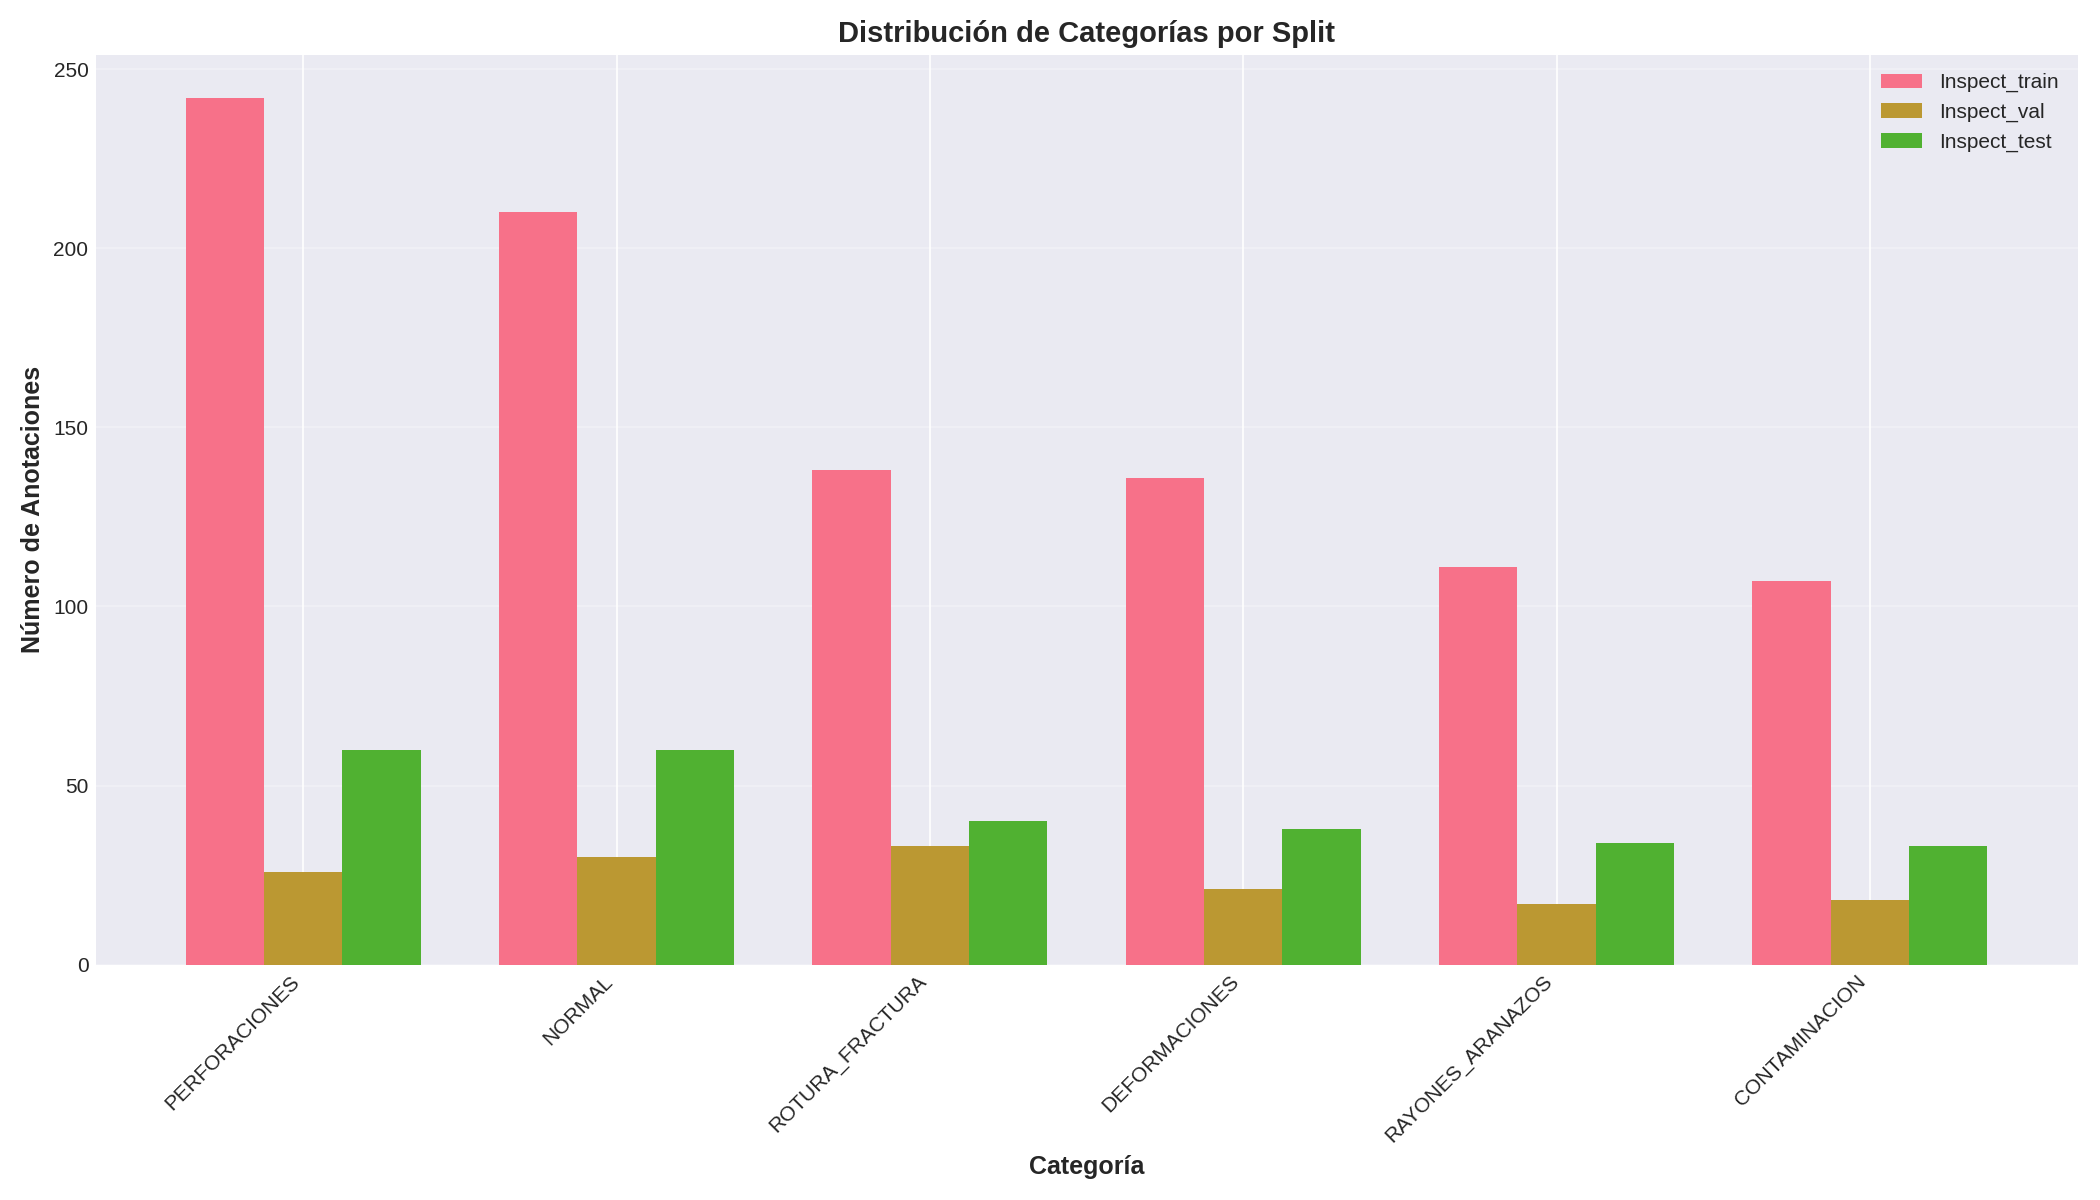
\includegraphics[width=0.95\textwidth]{fig/fase0_category_distribution.png}
\caption{Distribución de anotaciones por categoría y partición en el conjunto de datos final balanceado.}
\label{fig:fase0_category_distribution}
\end{figure}

\begin{figure}[htbp]
\centering
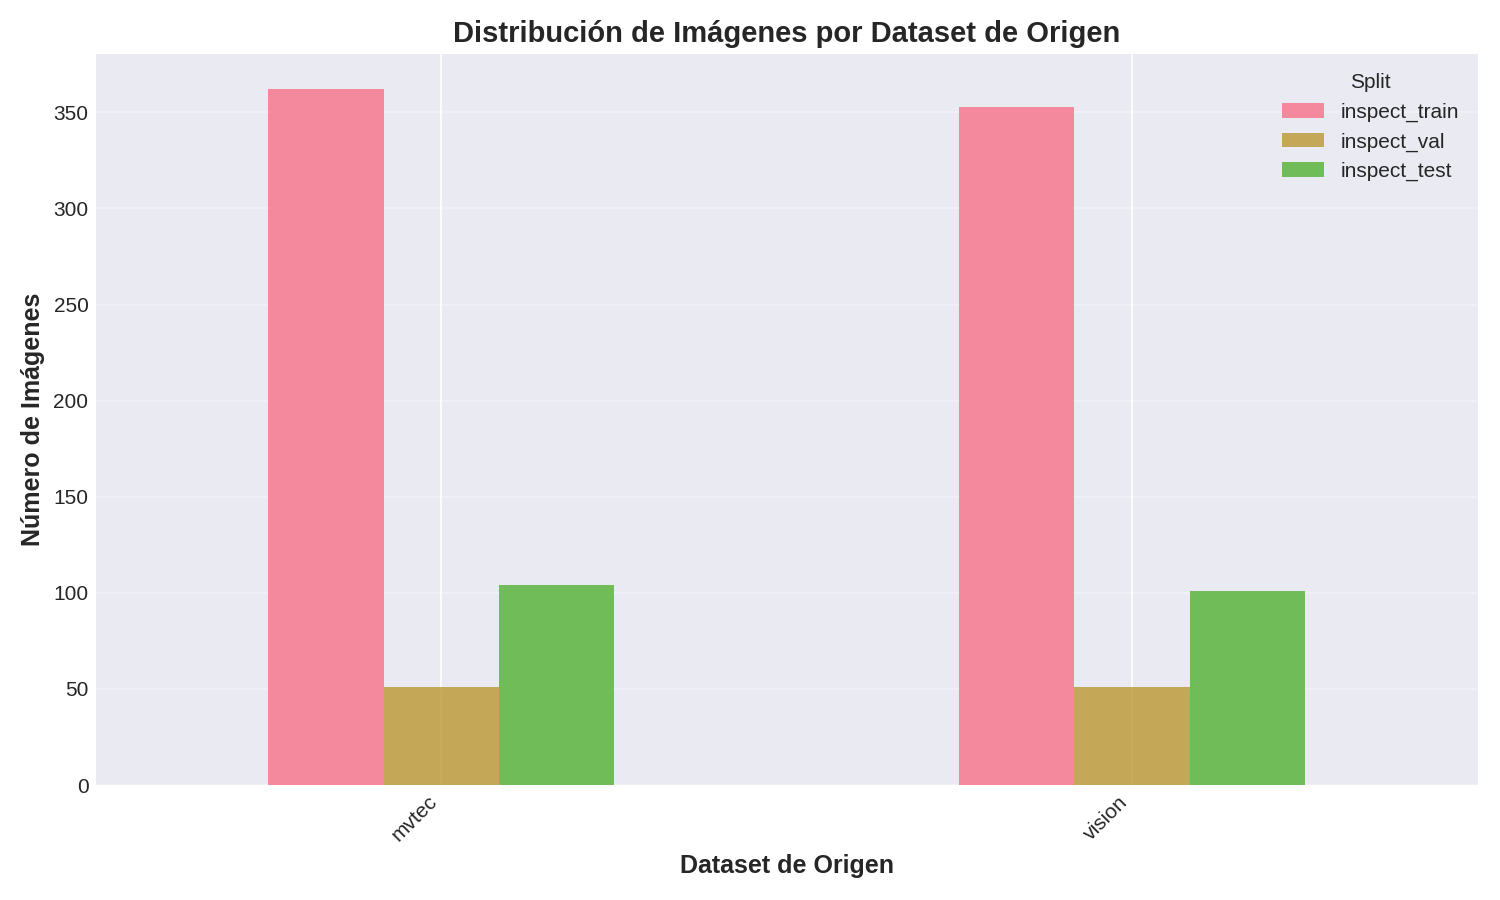
\includegraphics[width=0.95\textwidth]{fig/fase0_source_dataset_distribution.png}
\caption{Distribución del número de imágenes por conjunto de datos de origen (MVTec AD vs VISION-Datasets) en el conjunto de datos final.}
\label{fig:fase0_source_dataset_distribution}
\end{figure}

\FloatBarrier
\subsubsection{Características de resolución y escalas}

El conjunto de datos presenta una variabilidad de resolución excepcionalmente alta (Figura~\ref{fig:fase0_image_size_distributions}). Las distribuciones de ancho y alto muestran una mediana en torno a 1650$\times$1350 píxeles, con una cola larga que alcanza resoluciones de hasta 3840$\times$3620 píxeles en las imágenes de mayor calidad. Al mismo tiempo, el extremo inferior del rango incluye imágenes de apenas 262$\times$192 píxeles, procedentes de capturas con menor resolución de sensor. La distribución del lado corto evidencia que la gran mayoría de imágenes supera los 640 píxeles en ambas dimensiones, lo que implica que una resolución de entrenamiento de 640$\times$640 preservaría la información de la mayoría de imágenes sin recorte excesivo; sin embargo, para imágenes con defectos de tamaño milimétrico, la pérdida de detalle al redimensionar desde resoluciones superiores podría dificultar la detección.

La Figura~\ref{fig:fase0_width_vs_height_scatter} muestra la dispersión ancho--alto de todas las imágenes del conjunto de datos, diferenciadas por partición. Se observa que los puntos se agrupan principalmente en torno a la diagonal (relación de aspecto próxima a 1:1 o 4:3), sin diferencias sistemáticas entre particiones: las tres nubes de puntos (entrenamiento, validación, prueba) se solapan en la misma región, confirmando que la estratificación fue adecuada y que no se introdujeron sesgos de resolución entre conjuntos.

Estas características tienen consecuencias directas sobre las decisiones de entrenamiento. Dado que todos los modelos requieren una resolución de entrada fija, fue necesario escalar y recortar las imágenes originales. Se evaluaron dos resoluciones: 640$\times$640 píxeles, habitual en detectores de objetos eficientes, y 1024$\times$1024 píxeles, que preserva más detalle fino a costa de mayor consumo de memoria y tiempo de entrenamiento. La elección entre ambas opciones constituye una de las variables experimentales analizadas en las Fases 1 y 2, y su impacto sobre el rendimiento se discute en la sección~\ref{subsec:metricas}.

\begin{figure}[htbp]
\centering
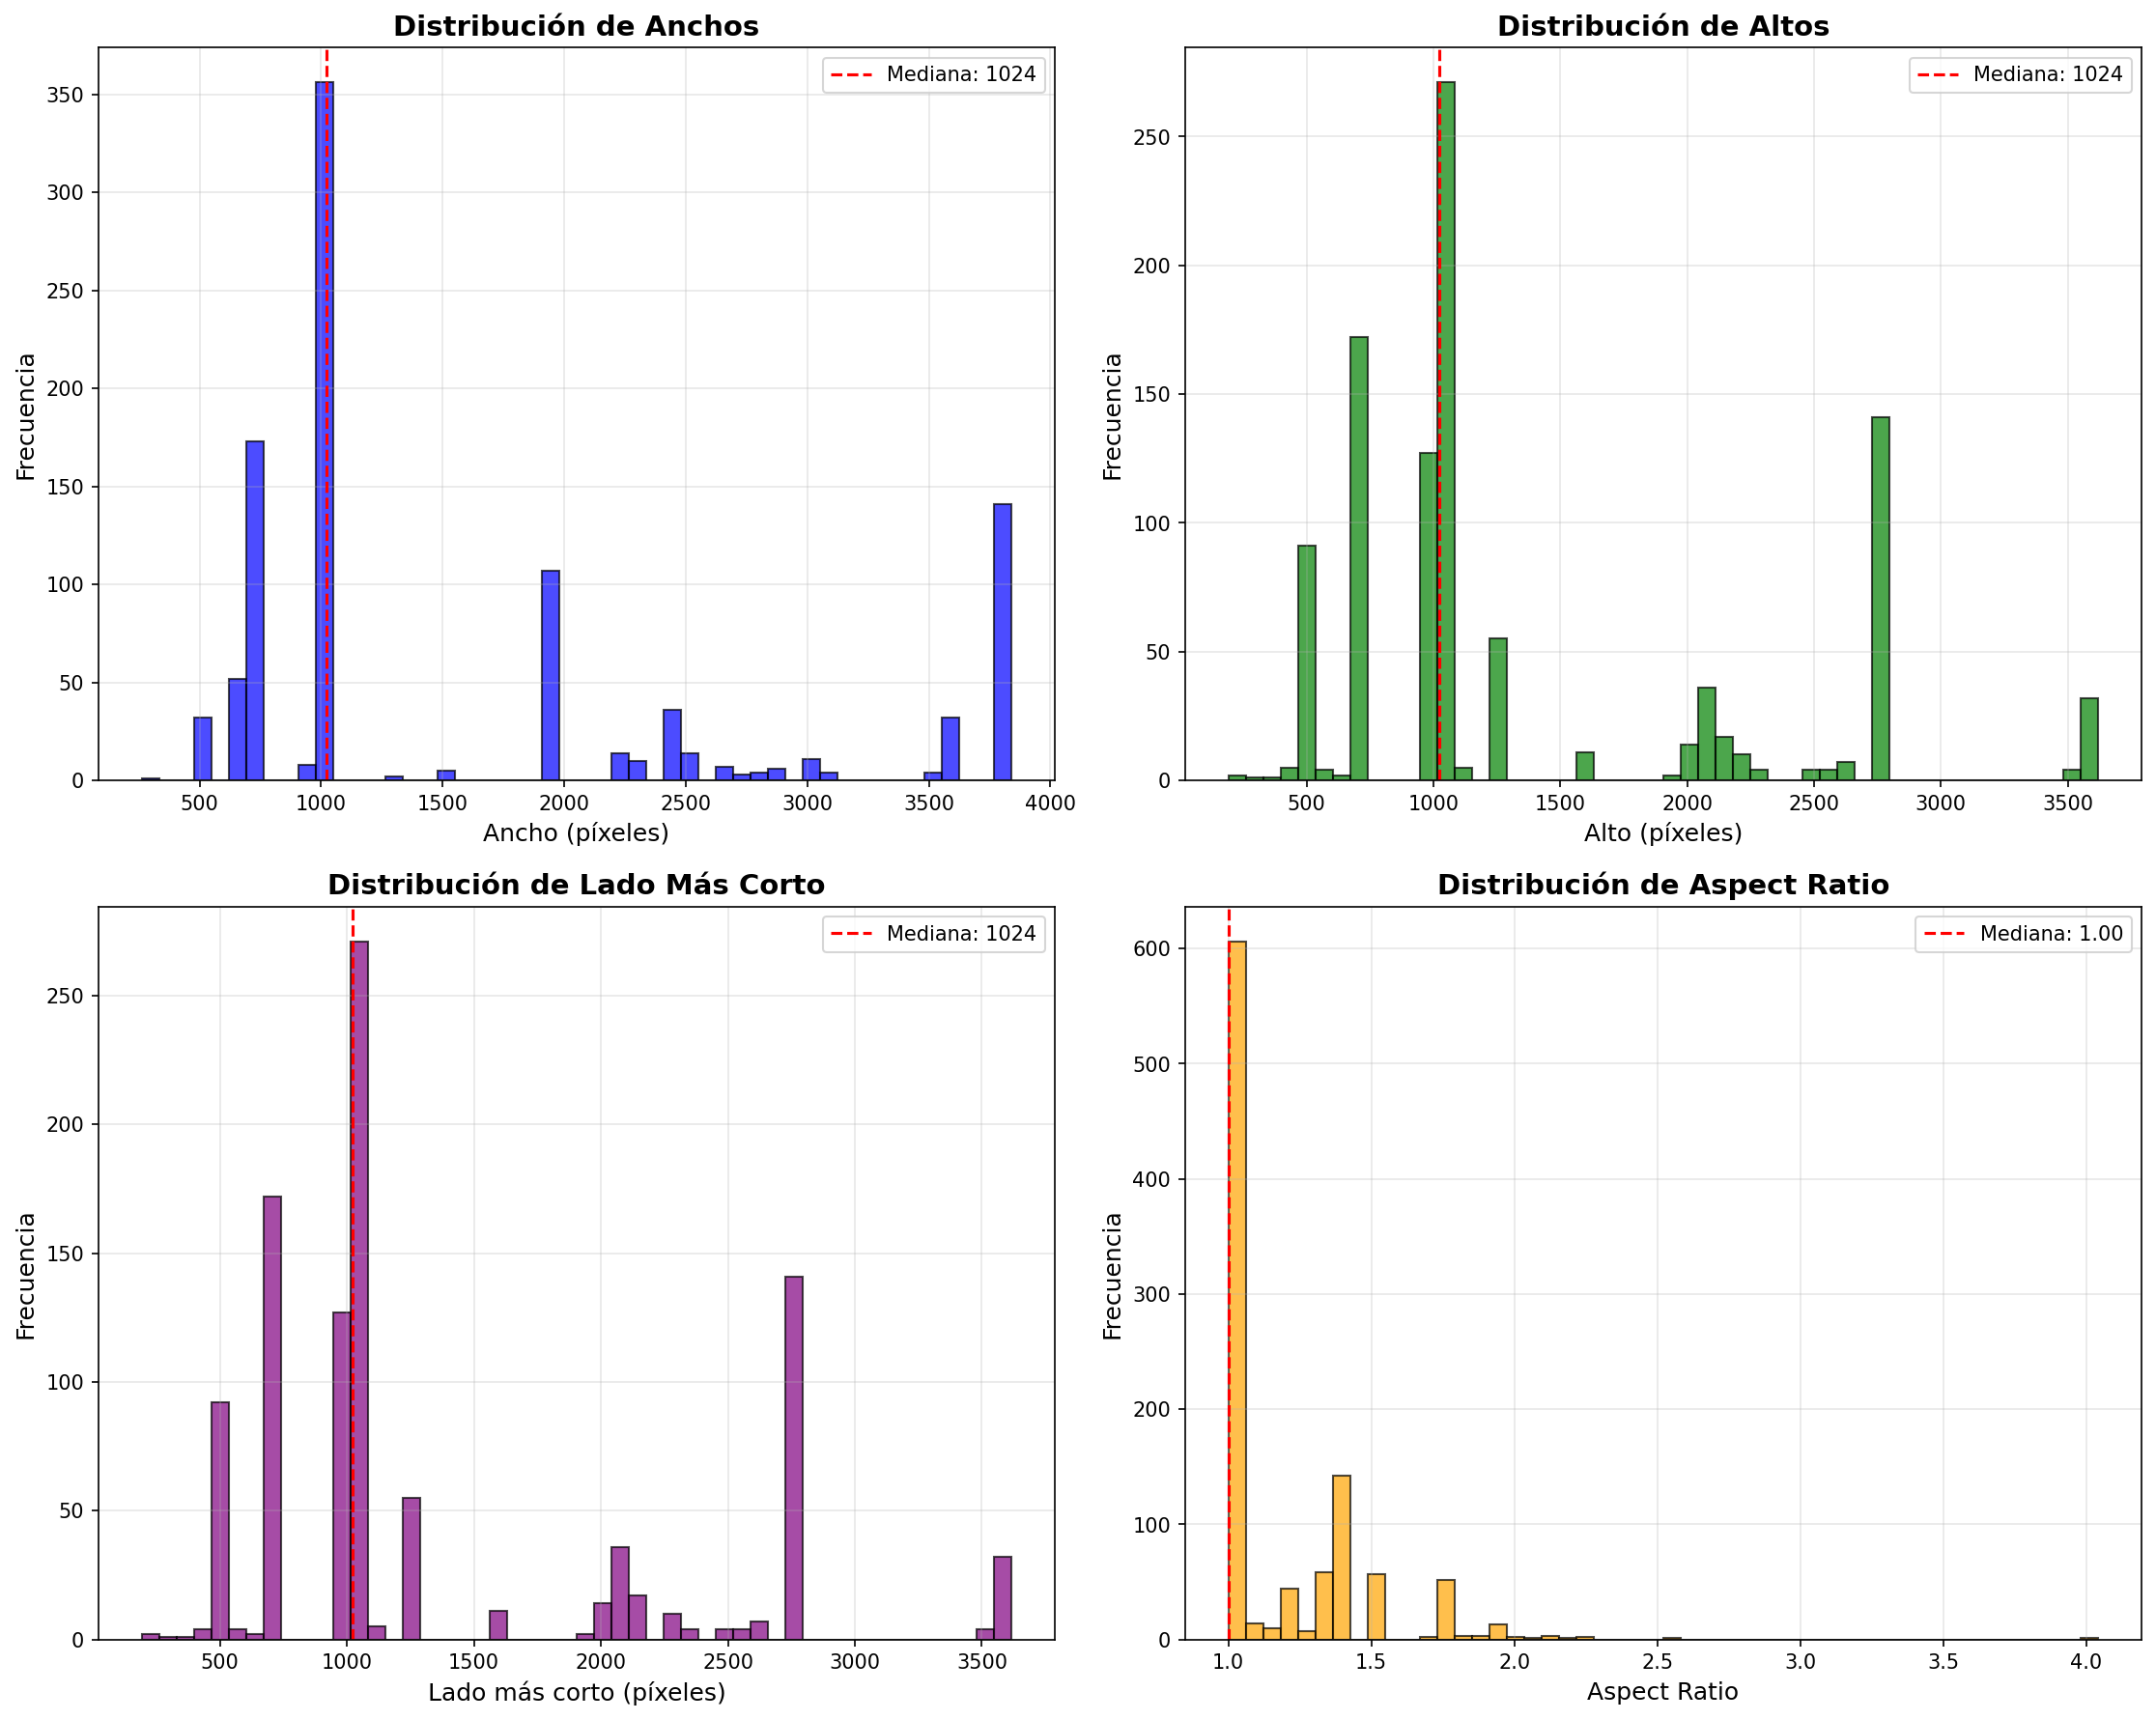
\includegraphics[width=0.95\textwidth]{fig/fase0_image_size_distributions.png}
\caption{Distribuciones de tamaños de imagen (ancho, alto, lado corto y relación de aspecto) en el conjunto de datos final.}
\label{fig:fase0_image_size_distributions}
\end{figure}

\begin{figure}[htbp]
\centering
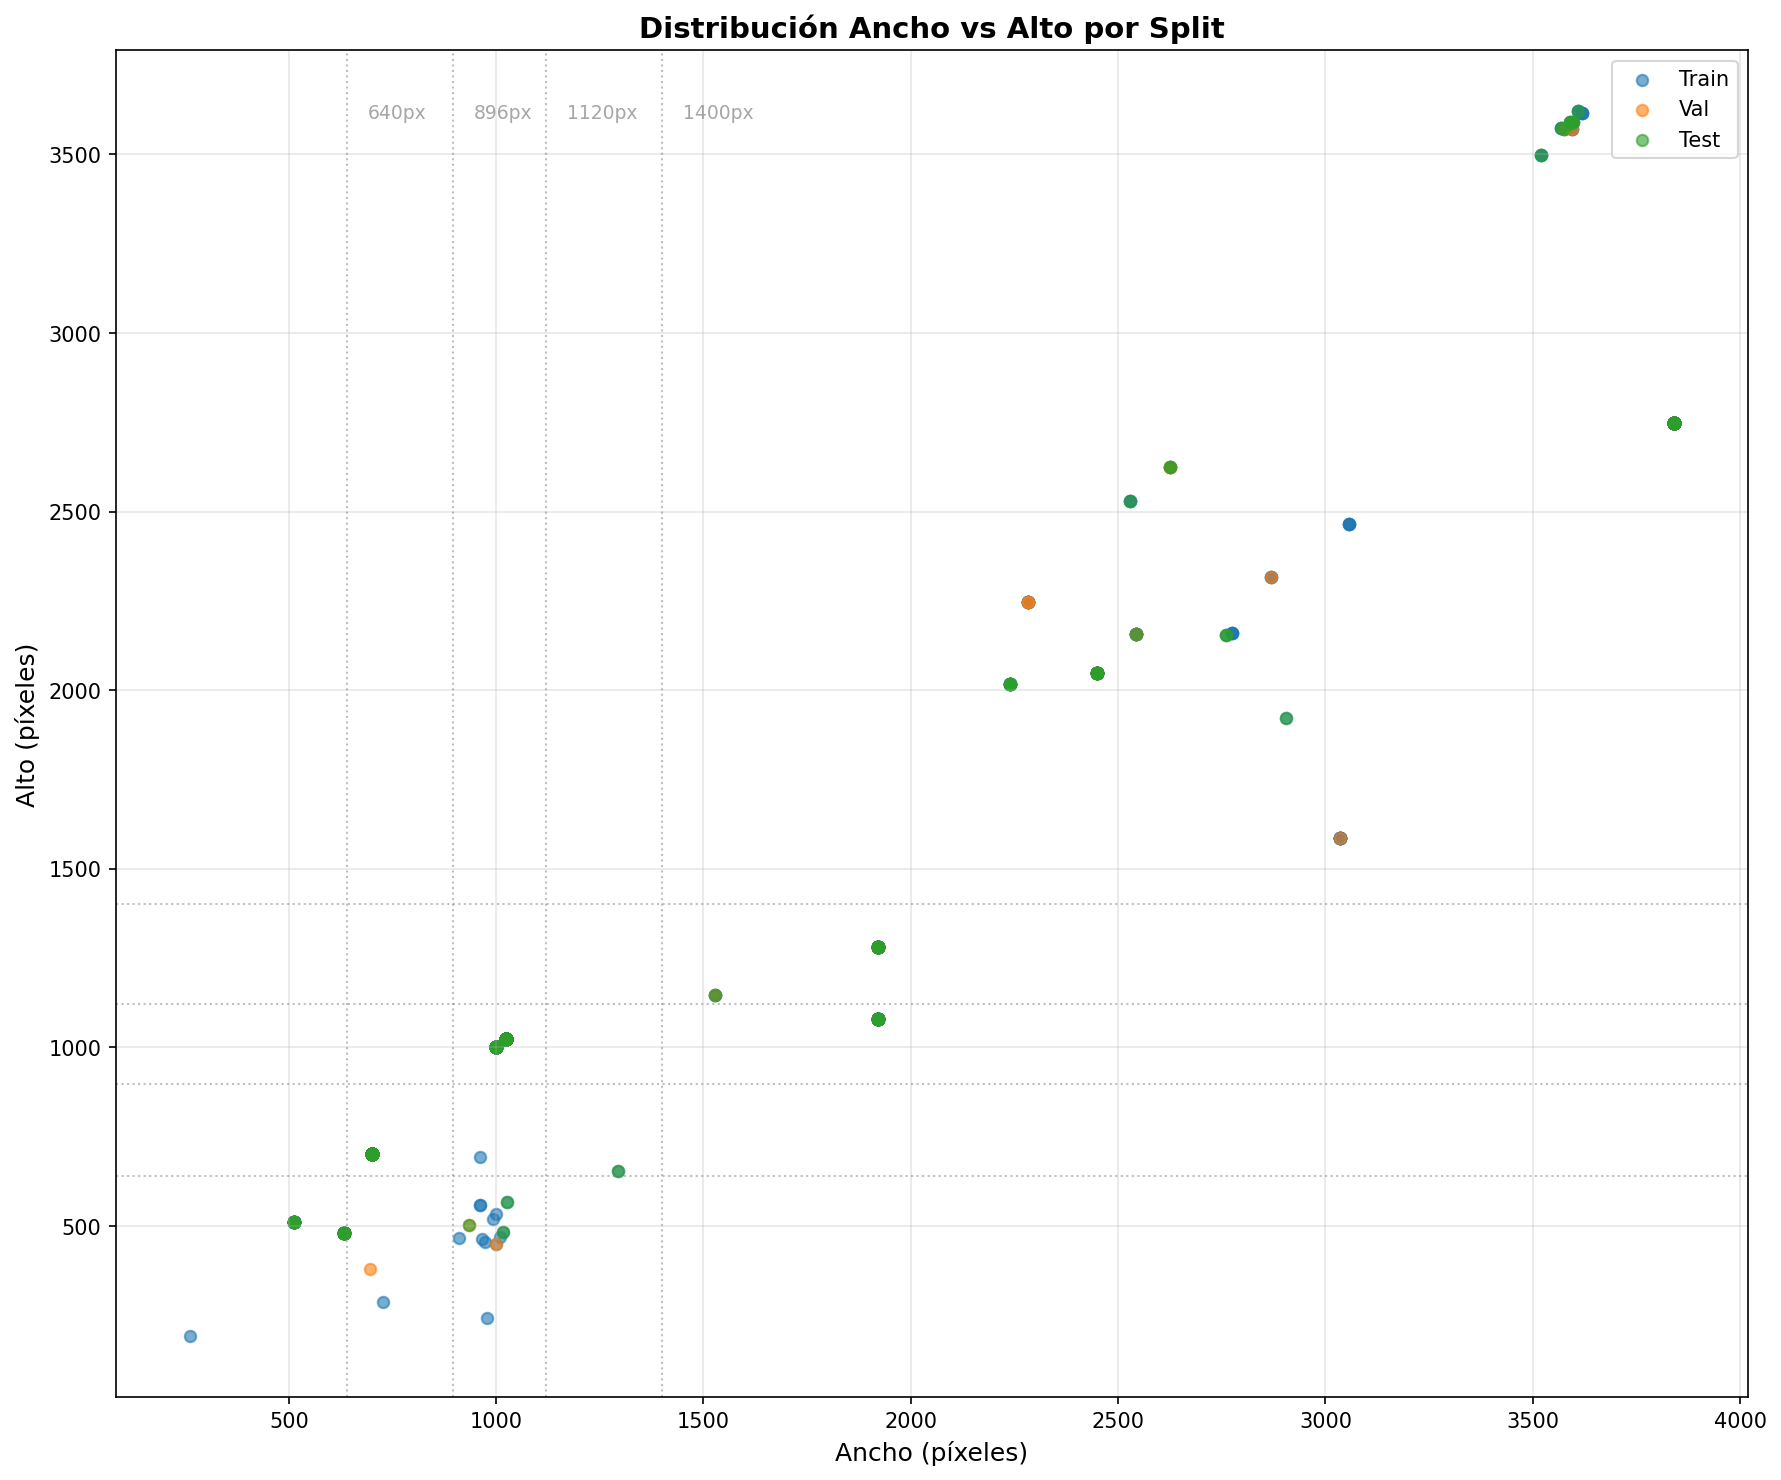
\includegraphics[width=0.95\textwidth]{fig/fase0_width_vs_height_scatter.png}
\caption{Dispersión ancho vs alto de las imágenes del conjunto de datos final, mostrando la variabilidad de resolución.}
\label{fig:fase0_width_vs_height_scatter}
\end{figure}

\FloatBarrier
\subsubsection{Características de las anotaciones (bounding boxes)}

El análisis de las cajas delimitadoras (Figura~\ref{fig:fase0_bbox_distribution}) muestra la existencia de una fracción relevante de cajas delimitadoras pequeñas. En la partición de entrenamiento, el 23.41\% de las cajas presenta anchura menor de 32 píxeles y el 22.25\% presenta altura menor de 32 píxeles (en validación y prueba estos porcentajes se sitúan entre el 16\% y el 20\%). Esta observación resulta especialmente relevante para modelos basados en Redes de Propuesta de Regiones (\textit{Region Proposal Networks}, RPN), cuyas anclas preconfiguradas operan habitualmente a escalas mínimas de 32 píxeles: cuando una caja delimitadora real es más pequeña que esa escala mínima, el modelo no es capaz de asociarla con ninguna ancla y la ignora durante el entrenamiento, reduciendo la sensibilidad del detector a defectos de tamaño reducido. Para mitigar este efecto, se contempló tanto el ajuste de la escala mínima de anclas como el aumento de la resolución de entrada, opción que se exploró en la Fase~3.

\begin{figure}[htbp]
\centering
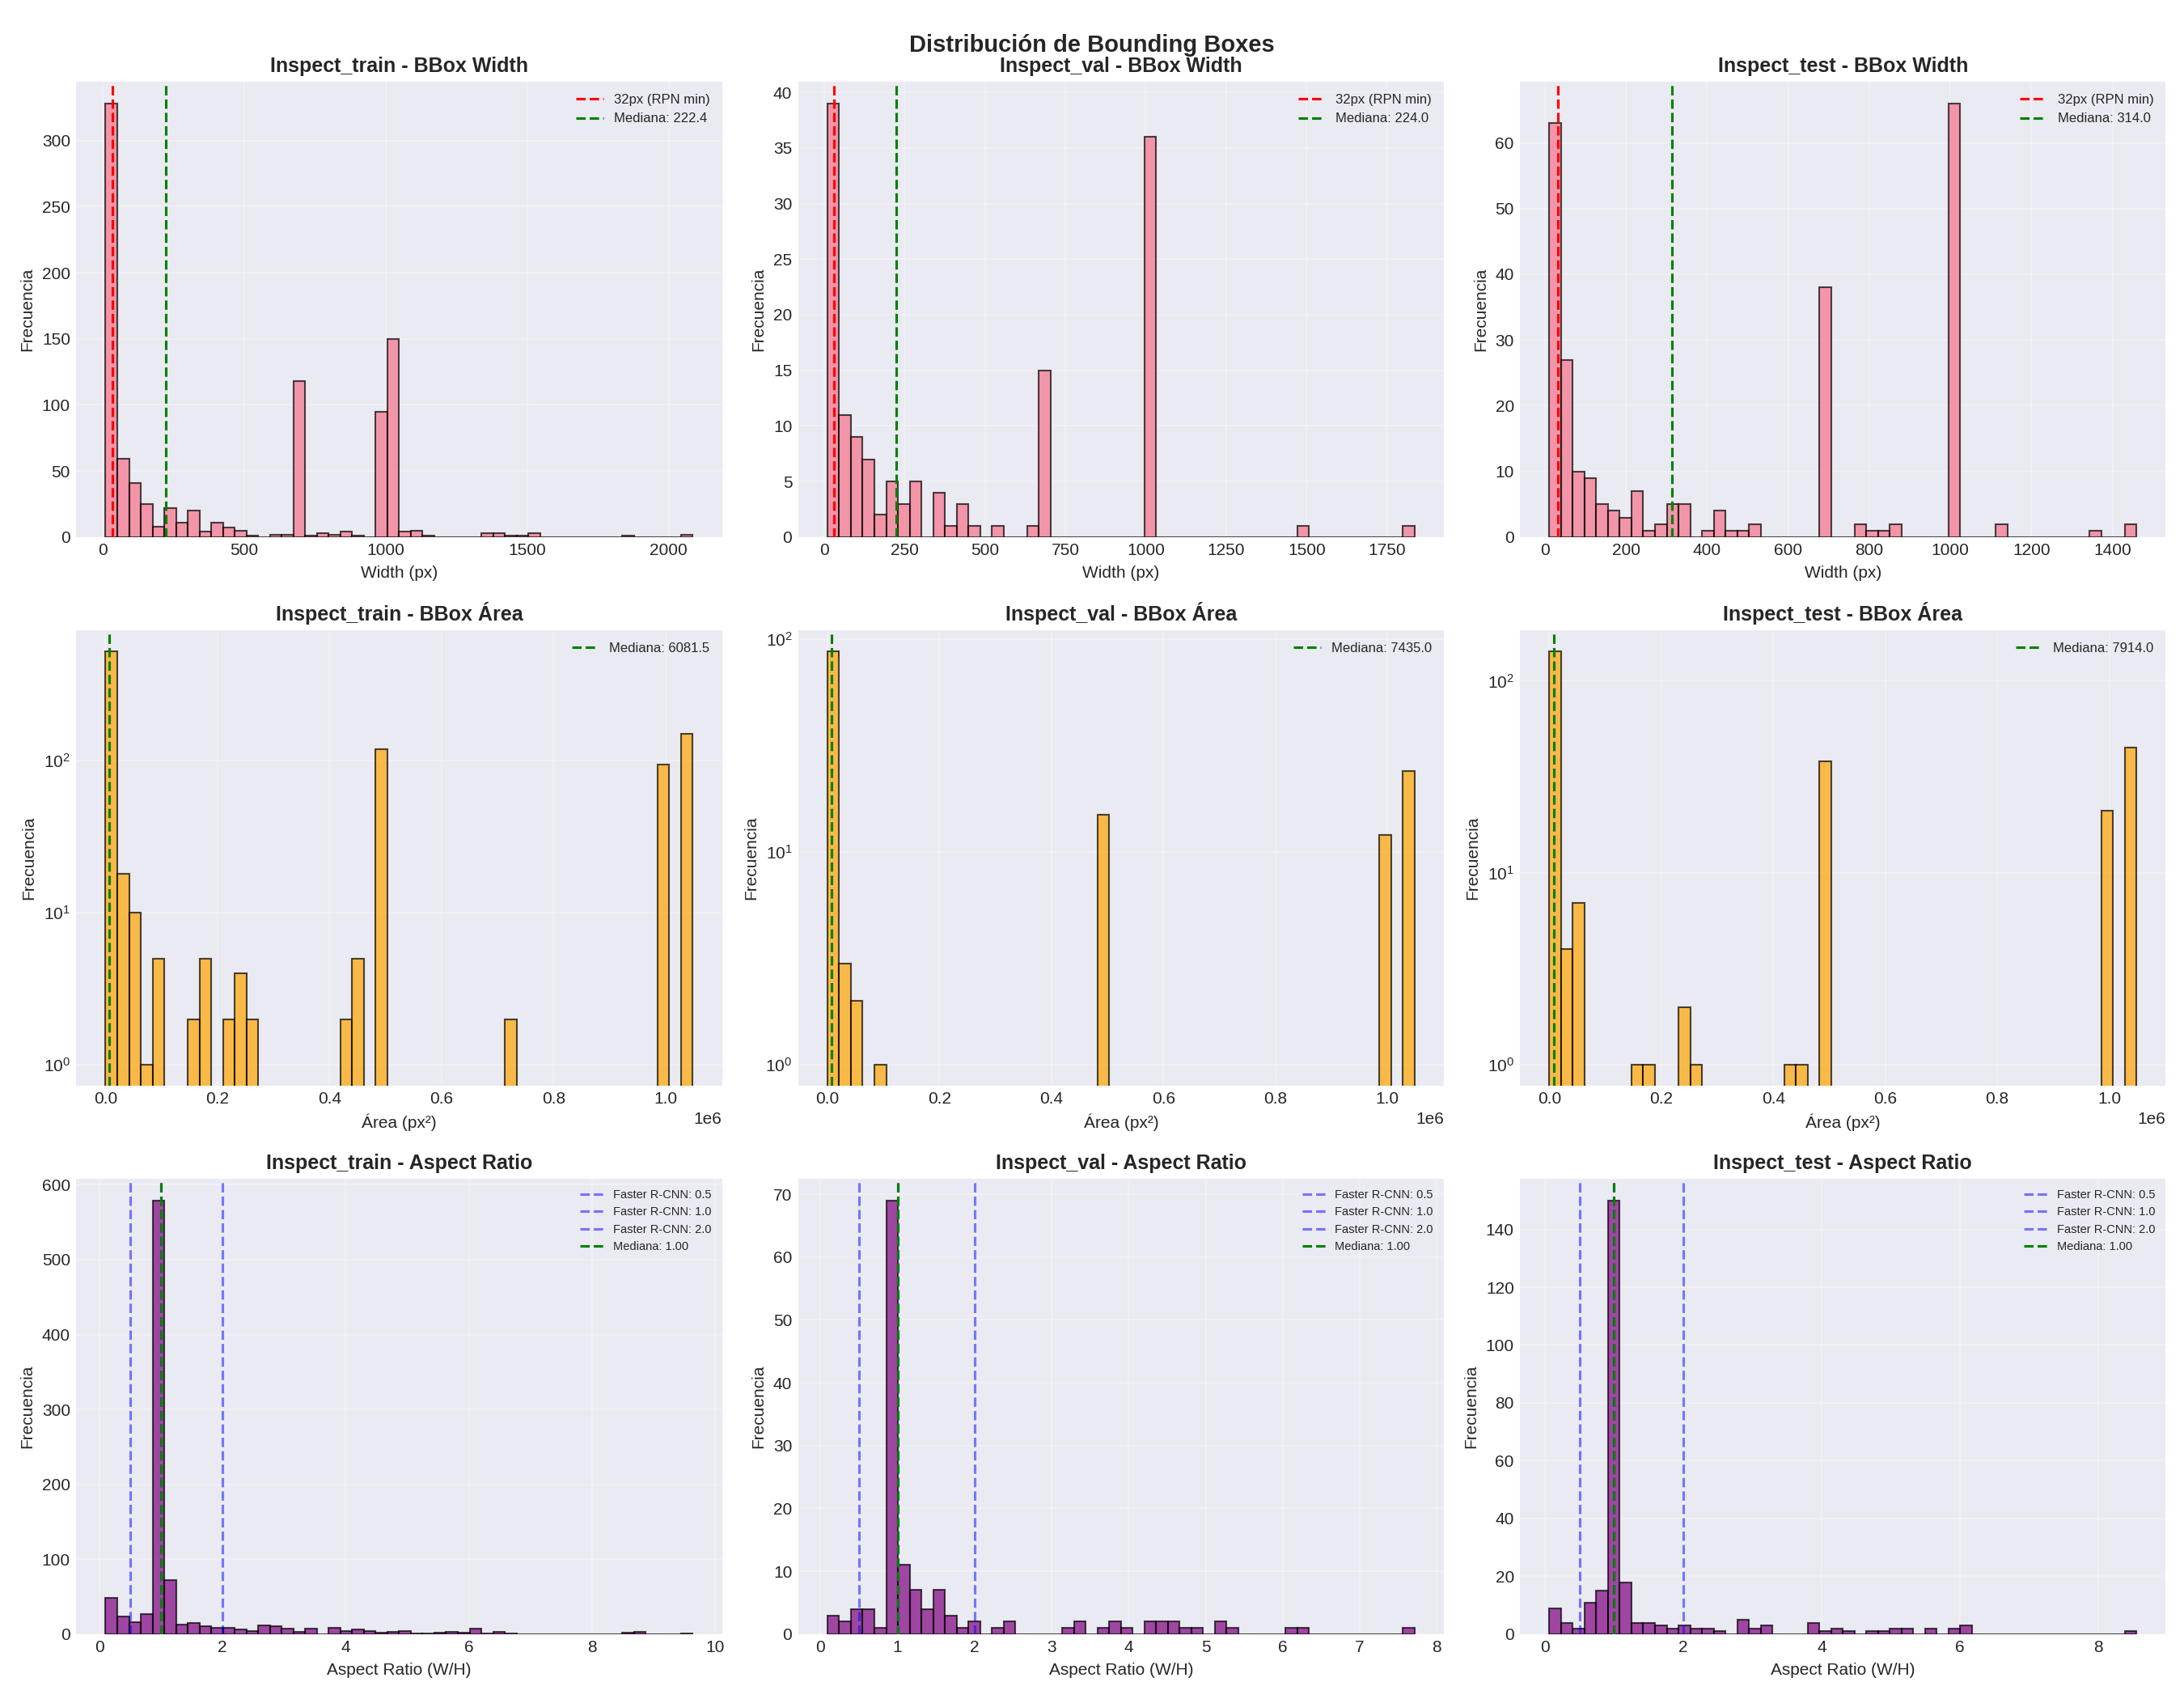
\includegraphics[width=0.95\textwidth]{fig/fase0_bbox_distribution.png}
\caption{Distribución de tamaños y relaciones de aspecto de las cajas delimitadoras en el conjunto de datos final.}
\label{fig:fase0_bbox_distribution}
\end{figure}

\FloatBarrier
\subsubsection{Balanceo mediante aumento}

Para mitigar el desbalance severo entre categorías (ratio inicial 24.5:1, con 1{,}039 imágenes de NORMAL frente a 58 de CONTAMINACIÓN), se implementó una estrategia híbrida de submuestreo y sobremuestreo complementada con aumento sintético conservador. El submuestreo (\textit{undersampling}) consiste en reducir el número de muestras de las clases mayoritarias para que no dominen el entrenamiento; el sobremuestreo (\textit{oversampling}) consiste en generar nuevas muestras artificiales de las clases minoritarias mediante transformaciones de imagen, de modo que el modelo vea más ejemplos de defectos poco frecuentes sin necesidad de nuevas capturas físicas. El uso combinado de ambas técnicas es una práctica consolidada en la literatura de visión por computador~\cite{wang2022defect}, ya que equilibra la distribución de clases respetando al mismo tiempo la semántica de las categorías deficitarias.

Las transformaciones aplicadas se seleccionaron cuidadosamente para preservar las características morfológicas de los defectos, descartando transformaciones agresivas (recorte aleatorio \textit{CutOut}, perspectiva severa, distorsión elástica) que podrían generar artefactos visuales o alterar patrones de textura relevantes para la discriminación de defectos finos:

\begin{itemize}
    \item \textbf{HorizontalFlip} ($p=0{,}5$): volteo horizontal, invariante a la simetría de los defectos superficiales en componentes electrónicos sin orientación forzada.
    \item \textbf{Rotate} ($\pm 5^{\circ}$, $p=0{,}5$): rotación restringida a $\pm 5$ grados para simular ligeras variaciones de orientación de captura sin alterar la morfología del defecto.
    \item \textbf{RandomBrightnessContrast} (límite $\pm 0{,}1$, $p=0{,}5$): variación mínima de brillo y contraste para reproducir diferencias de iluminación entre capturas sin saturar ni oscurecer texturas diagnósticas.
    \item \textbf{GaussNoise} (varianza 5--15, $p=0{,}3$): ruido gaussiano de baja intensidad para mejorar la robustez del modelo ante el ruido inherente al sensor de cámara industrial.
\end{itemize}

Se generaron en total 368 imágenes aumentadas, afectando principalmente a PERFORACIONES (+246 imágenes), DEFORMACIONES (+111) y CONTAMINACIÓN (+100), con contribuciones menores a \mbox{ROTURA\_FRACTURA} (+60) y \mbox{RAYONES\_ARAÑAZOS} (+58). El resultado fue un conjunto de datos con ratio máx/mín de 2.08:1, dentro del umbral recomendado para entrenamiento supervisado ($< 3{:}1$). La proporción de imágenes aumentadas se mantuvo homogénea entre particiones (35.9\% en entrenamiento, 38.2\% en validación y 35.1\% en prueba), garantizando que no se introdujo correlación espuria entre particiones. La Figura~\ref{fig:fase0_augmentation_distribution} muestra esta distribución.

\begin{figure}[htbp]
\centering
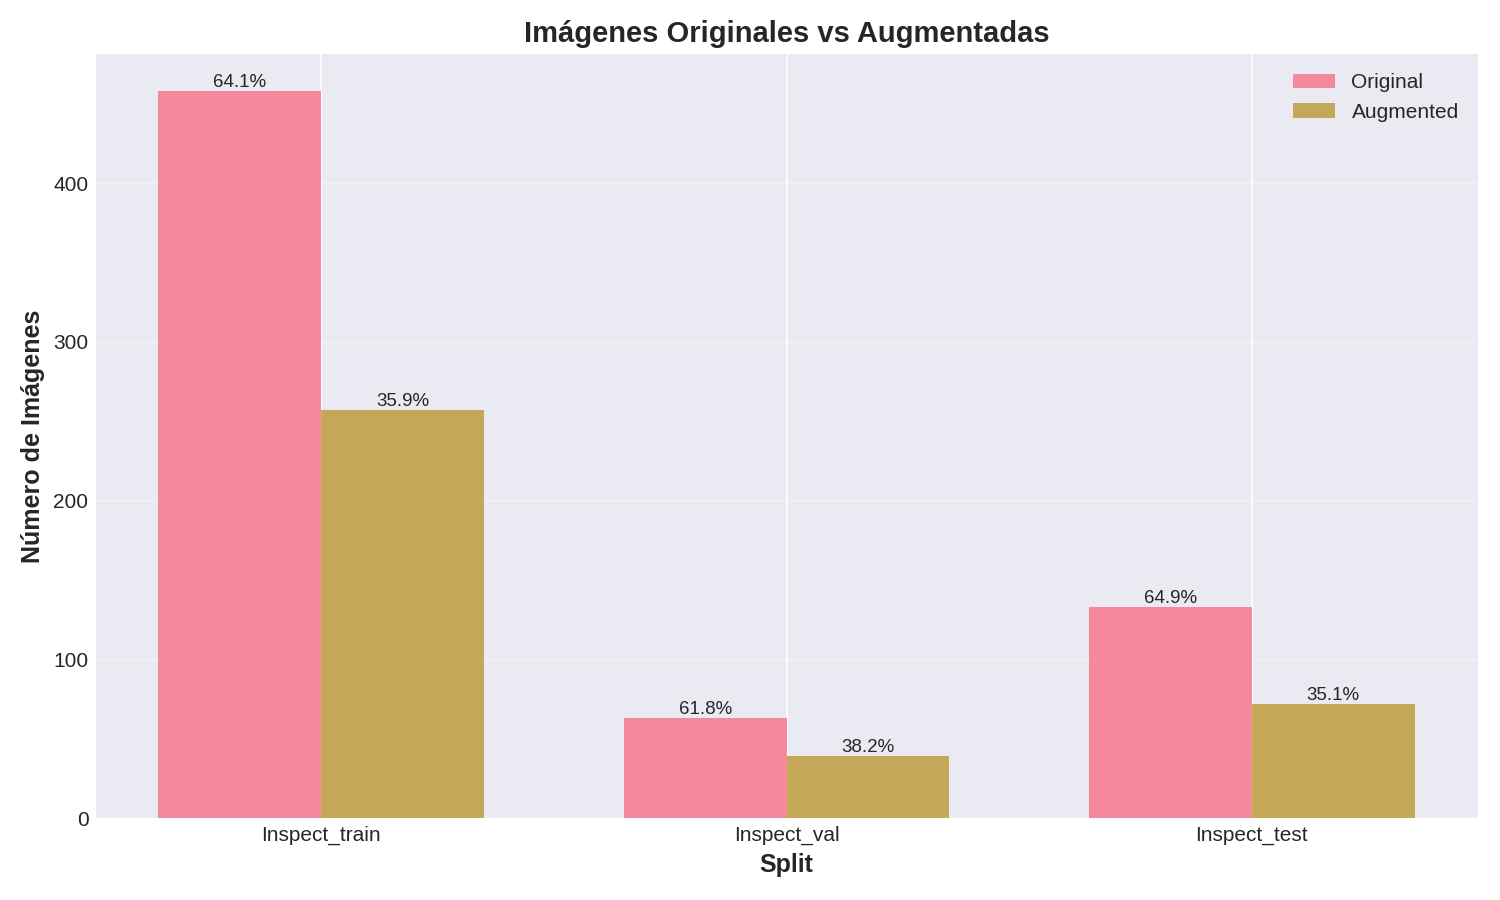
\includegraphics[width=0.95\textwidth]{fig/fase0_augmentation_distribution.png}
\caption{Proporción de imágenes originales y aumentadas por partición en el conjunto de datos final. La homogeneidad inter-partición ($\sim$36\%) confirma que el aumento no introduce sesgo en la evaluación.}
\label{fig:fase0_augmentation_distribution}
\end{figure}

\FloatBarrier
\subsection{Conclusiones de la preparación del conjunto de datos}

El proceso de curación (Etapas 1--5) permitió transformar dos fuentes heterogéneas en un conjunto de datos único, trazable y listo para experimentación:
\begin{itemize}
    \item Se obtuvo un conjunto de datos final de 1{,}022 imágenes y 1{,}354 anotaciones, con 6 categorías unificadas.
    \item El balance entre clases se estabilizó hasta un ratio máx/mín de 2.08:1, adecuado para entrenamiento supervisado.
    \item Se validó estadísticamente la estratificación de particiones ($p=0.999$) y la ausencia de fugas entre particiones.
    \item El análisis de escalas evidenció la presencia de cajas delimitadoras pequeñas y alta variabilidad de resolución, aspectos que influyeron en las decisiones de configuración del entrenamiento.
\end{itemize}

\section{Metodología de trabajo}
\label{sec:metodologia}

Una vez preparado el conjunto de datos (sección~\ref{sec:preparacion_dataset}), se realizó una experimentación sistemática con diferentes arquitecturas. El presente trabajo se ha estructurado siguiendo una metodología experimental rigurosa, fundamentada en el método científico y adaptada a las particularidades de la investigación en aprendizaje profundo. La aproximación metodológica se caracteriza por:

\begin{enumerate}
    \item \textbf{Enfoque iterativo e incremental}: El desarrollo se ha organizado en fases sucesivas, donde cada iteración construye sobre los resultados y lecciones aprendidas de la anterior. Esta aproximación permite identificar problemas de forma temprana y ajustar la estrategia de forma adaptativa.
    
    \item \textbf{Comparación sistemática y controlada}: Todas las arquitecturas y configuraciones se han evaluado bajo condiciones experimentales equivalentes, utilizando el mismo conjunto de datos, el mismo conjunto de prueba (205 imágenes) y las mismas métricas de evaluación. Esta consistencia garantiza que las diferencias observadas se atribuyan a las variaciones arquitectónicas o de configuración, no a factores externos.
    
    \item \textbf{Validación científica rigurosa}: Se ha implementado un protocolo de validación que incluye:
    \begin{enumerate}
        \item Separación estricta entre conjuntos de entrenamiento, validación y prueba.
        \item Uso del conjunto de prueba únicamente para evaluación final.
        \item Selección del mejor modelo guardado basada en métricas de validación. Durante el entrenamiento, el sistema almacena periódicamente el estado completo de los pesos del modelo; al concluir, se selecciona el estado guardado con mayor precisión media global (mAP, \textit{mean Average Precision})@0.5 en el conjunto de validación como modelo final para la evaluación sobre el conjunto de prueba.
        \item Documentación exhaustiva de todas las configuraciones experimentales.
    \end{enumerate}
    
    \item \textbf{Análisis evolutivo}: Se ha realizado un seguimiento detallado de la evolución del rendimiento a lo largo de múltiples iteraciones, permitiendo identificar patrones de convergencia, puntos óptimos y compromisos entre diferentes configuraciones.
\end{enumerate}

\subsection{Conjunto de datos y configuración experimental}

El conjunto de datos utilizado en todos los experimentos es el conjunto industrial curado descrito en la sección~\ref{sec:preparacion_dataset}, compuesto por imágenes de componentes manufacturados con anotaciones de defectos en formato COCO. Sus características principales son:

\begin{itemize}
    \item \textbf{Resolución original}: Mediana de aproximadamente 1650×1350 píxeles, con variabilidad significativa entre imágenes.
    \item \textbf{Conjunto de prueba}: 205 imágenes, utilizado exclusivamente para evaluación final y nunca durante el entrenamiento o selección de hiperparámetros.
    \item \textbf{Categorías de defectos}: Seis clases en total: NORMAL (sin defectos), DEFORMACIONES, \mbox{ROTURA\_FRACTURA}, \mbox{RAYONES\_ARAÑAZOS}, PERFORACIONES y CONTAMINACIÓN.
    \item \textbf{Variabilidad}: El conjunto de datos presenta alta variabilidad en términos de iluminación, tipos de superficies, escalas de defectos y condiciones de captura, lo que lo convierte en un conjunto de referencia desafiante y realista.
\end{itemize}

\subsection{Métricas de evaluación}
\label{subsec:metricas}

La evaluación de todos los modelos se ha realizado utilizando el protocolo estándar COCO. A continuación se presenta una descripción técnica precisa de cada métrica, necesaria para interpretar correctamente los resultados comparativos entre arquitecturas.

\subsubsection{Intersección sobre unión (IoU)}

La \acrfull{IoU} mide el solapamiento geométrico entre una caja delimitadora predicha $B_p$ y la caja de referencia (\textit{ground truth}) $B_{gt}$:
\begin{equation}
\text{IoU}(B_p, B_{gt}) = \frac{|B_p \cap B_{gt}|}{|B_p \cup B_{gt}|}
\label{eq:iou}
\end{equation}
Una predicción se considera un \acrfull{TP} si $\text{IoU} \geq \theta$, donde $\theta$ es el umbral de IoU establecido (en este trabajo, $\theta = 0.5$). Si $\text{IoU} < \theta$, la predicción se clasifica como \acrfull{FP}.

\subsubsection{Precisión y sensibilidad (\textit{recall}) por clase}

Para cada categoría de defecto, la precisión representa la fracción de las detecciones realizadas que son correctas:
\begin{equation}
\text{Precisión} = \frac{\text{TP}}{\text{TP} + \text{FP}}
\label{eq:precision}
\end{equation}
La sensibilidad mide la fracción de las instancias reales que el modelo ha detectado correctamente:
\begin{equation}
\text{Sensibilidad} = \frac{\text{TP}}{\text{TP} + \text{FN}}
\label{eq:recall}
\end{equation}
donde \acrshort{FN} es el número de instancias reales no detectadas. Estas dos métricas presentan un compromiso inherente: umbrales de confianza bajos aumentan la sensibilidad, pero reducen la precisión, y viceversa.

\subsubsection{Precisión media (AP) por clase}

La \acrfull{AP} (precisión media en castellano) por clase integra el compromiso entre precisión y sensibilidad a lo largo de todos los umbrales de confianza posibles, computando el área bajo la curva precisión--exhaustividad (precisión--sensibilidad):
\begin{equation}
\text{AP} = \int_0^1 p(r)\, \mathrm{d}r \approx \sum_{k=1}^{n} p(r_k) \cdot \Delta r_k
\label{eq:ap}
\end{equation}
donde $p(r)$ es la precisión cuando la sensibilidad es $r$ y la suma discreta aproxima el área con $n$ puntos de la curva. La AP es más informativa que un único par (Precisión, Sensibilidad) porque captura el comportamiento del modelo en todo el rango operativo de umbrales de confianza. En este trabajo se reporta AP@0.5, es decir, AP calculada con el umbral de IoU fijado en 0.5.

La evaluación por clase se ha priorizado como métrica principal frente al mAP global porque permite identificar el comportamiento del modelo en cada tipo específico de defecto. Esto es fundamental en un sistema de inspección industrial, donde el rendimiento en las categorías más críticas (\mbox{ROTURA\_FRACTURA}, PERFORACIONES) puede tener mayor relevancia operativa que el promedio global.

\subsubsection{Precisión media global (mAP@0.5)}

La \acrfull{mAP}@0.5 es el promedio aritmético de los valores de AP@0.5 de todas las clases:
\begin{equation}
\text{mAP@0.5} = \frac{1}{C} \sum_{c=1}^{C} \text{AP}_c
\label{eq:map}
\end{equation}
donde $C$ es el número de categorías. En este trabajo se ha utilizado $C = 6$ categorías. Esta métrica constituye el indicador global del rendimiento del detector y es la referencia principal para la comparativa entre arquitecturas.

\subsubsection{Umbral de confianza y consideraciones sobre la comparativa}

Todos los modelos han sido evaluados aplicando un umbral de confianza de puntuación de $0.15$. Esta elección no es arbitraria: durante los experimentos con arquitecturas CNN (ResNet-18 y EfficientNet-B0), se observó que estas redes producen un número muy reducido de detecciones y, en los casos en que detectan objetos, lo hacen con puntuaciones de confianza bajos, frecuentemente inferiores a 0.3. Aplicar un umbral más estricto (como 0.5, habitual en la literatura) habría eliminado prácticamente todas las detecciones de las CNNs, haciendo inviable cualquier comparativa cuantitativa.

Por consiguiente, se estableció un umbral $0.15$ como el umbral más permisivo que permite a las arquitecturas CNN producir detecciones medibles, garantizando una comparativa justa entre paradigmas. Esta decisión beneficia sistemáticamente a las CNNs (se aceptan sus detecciones de baja confianza), lo que hace que el rendimiento superior demostrado por DEIMv2 sea aún más significativo.

\subsubsection{Consideraciones sobre precisión = 1.0 en DEIMv2}

Un resultado que requiere justificación explícita es la precisión de 1.0 (100\%) reportada en todas las clases para todos los experimentos con DEIMv2. Este resultado no es un artefacto computacional ni indica sobreajuste; es una consecuencia directa de la alta capacidad discriminativa de la arquitectura.

DEIMv2, gracias a las representaciones semánticas ricas de DINOv3, genera un número sustancialmente mayor de detecciones que las CNNs. Crucialmente, la arquitectura es capaz de producir siempre al menos una detección por encima del umbral de 0.15 que coincide geométricamente (IoU $\geq$ 0.5) y semánticamente con una instancia real de la clase correspondiente. En términos de la ecuación~\eqref{eq:precision}, esto significa que el número de \acrshort{FP} por encima del umbral de confianza seleccionado es nulo o despreciable: todas las cajas que el modelo reporta con confianza superior a 0.15 corresponden a instancias reales. Esta situación refleja que el modelo ha aprendido a asignar puntuaciones altas solo a regiones de la imagen que efectivamente contienen defectos, resultado consistente con la validación en la Fase 4 a umbrales más estrictos (0.75 y 0.90), donde la precisión se mantiene elevada.

\subsection{Criterios de selección del mejor modelo guardado}

Se han establecido criterios diferenciados según la arquitectura:

\begin{itemize}
    \item \textbf{Arquitecturas CNN (ResNet-18, EfficientNet)}: Selección basada en menor pérdida de validación (\texttt{val\_loss}), criterio estándar para modelos Faster R-CNN, donde la pérdida de validación correlaciona bien con el rendimiento en detección.
    \item \textbf{Vision Transformers (DEIMv2)}: Selección basada en mayor mAP@0.5 en el conjunto de validación, ya que esta métrica captura de forma más directa el rendimiento de detección de objetos. En arquitecturas DETR, la pérdida de entrenamiento no siempre correlaciona con el mAP, lo que hace preferible usar la métrica de detección directamente.
\end{itemize}

La evaluación final de todos los modelos se realiza exclusivamente sobre el subconjunto de prueba (205 imágenes), que no ha sido utilizado en ningún caso durante el proceso de entrenamiento y selección de hiperparámetros. Esta separación estricta garantiza que las métricas reportadas reflejen la capacidad de generalización real del modelo y no la memorización de los datos de entrenamiento.


\section{Planificación en fases experimentales}
\label{sec:planificacion}

El desarrollo experimental se ha estructurado en cuatro fases principales, cada una con objetivos específicos y metodología adaptada. Nótese que la preparación del conjunto de datos (sección~\ref{sec:preparacion_dataset}) constituye un bloque previo e independiente; las fases que se enumeran a continuación corresponden exclusivamente a la experimentación con modelos:

\begin{description}
    \item[\textbf{Fase 1: Línea base con arquitecturas CNN}] Establecer líneas base con arquitecturas convolucionales tradicionales (ResNet-18 y EfficientNet-B0). El fracaso de estos modelos (mAP 0.077 y 0.162) actuará como motor de búsqueda que justifica explorar arquitecturas alternativas.
    
    \item[\textbf{Fase 2: Exploración de Vision Transformers}] Evaluar el rendimiento de DEIMv2, explorando resoluciones (640px vs 1024px) y épocas (80, 120, 300) hasta identificar el punto óptimo de convergencia (época 187 de 300).
    
    \item[\textbf{Fase 3: Validación experimental}] Experimento crucial: re-entrenar las CNNs a 1024×1024 bajo las mismas condiciones que DEIMv2 para demostrar que la mejora se debe a la arquitectura Vision Transformer y no a la resolución de entrada.
    
    \item[\textbf{Fase 4: Validación de robustez}] Evaluar el mejor modelo con umbrales de confianza más estrictos (0.75 y 0.90) para descartar sobreajuste y verificar que la precisión observada no es consecuencia del umbral bajo.
\end{description}

Esta estructura permite una comparación justa y rigurosa entre arquitecturas, garantizando que las conclusiones extraídas sean válidas y reproducibles.

Con la planificación establecida, se presenta a continuación la ejecución de cada fase experimental, comenzando por las líneas base con arquitecturas convolucionales.

\section{Fase 1: Línea base con arquitecturas CNN}
\label{sec:fase1}

Esta sección documenta la primera fase experimental del trabajo, cuyo objetivo es establecer una referencia de rendimiento con arquitecturas convolucionales clásicas sobre el conjunto de datos curado. Se entrenan dos detectores de objetos basados en Faster R-CNN~\cite{ren_faster_2016}: uno con la red base ResNet-18~\cite{he2016resnet} y otro con EfficientNet-B0~\cite{tan2019efficientnet}, ambos a la resolución nativa de las imágenes del conjunto de datos. Los resultados de esta fase definen el nivel de rendimiento que la arquitectura Vision Transformer debe superar para justificar su adopción, y sirven de punto de comparación directo en las fases posteriores. La sección incluye la justificación de los hiperparámetros empleados, la descripción de cada experimento y el análisis de los resultados obtenidos.

\subsection{Motivación y objetivos}

La descripción conceptual de ResNet-18 y EfficientNet-B0 se presenta en la sección~\ref{subsec:cnn-arquitecturas-referencia}; aquí se reproducen sus diagramas de arquitectura como referencia visual para contextualizar los experimentos. Las Figuras~\ref{fig:diagrama-resnet18} y~\ref{fig:diagrama-efficientnet}, adaptadas de sus respectivos artículos originales~\cite{he2016resnet,tan2019efficientnet}, ilustran los bloques estructurales clave de cada red.

\begin{figure}[H]
\centering

\includegraphics[width=0.85\textwidth]{diagramas-arquitectura/resnet18-arquitetcura-diagrama.png}
\caption{Arquitectura ResNet-18. Adaptado de He et al.~\cite{he2016resnet}.}
\label{fig:diagrama-resnet18}
\end{figure}

\begin{figure}[H]
\centering

\includegraphics[width=0.85\textwidth]{diagramas-arquitectura/efficientnet-diagrama-arquitetcura.png}
\caption{Arquitectura EfficientNet-B0. Adaptado de Tan y Le~\cite{tan2019efficientnet}.}
\label{fig:diagrama-efficientnet}
\end{figure}

El objetivo de esta fase consiste en evaluar el rendimiento de estas arquitecturas en el problema específico de detección de defectos industriales sin modificaciones especiales, utilizando las imágenes en su resolución nativa para maximizar la información visual disponible.

\subsection{Justificación de los hiperparámetros de entrenamiento para arquitecturas CNN}
\label{subsec:justificacion_hiperparametros_cnn}

La selección de hiperparámetros para las arquitecturas CNN responde a principios establecidos en la literatura de detección de objetos con Faster R-CNN~\cite{ren_faster_2016} y a las particularidades de cada red base. A continuación se justifican los valores empleados en cada experimento.

\paragraph{ResNet-18. Optimizador: SGD con momentum 0.9.}
SGD (Stochastic Gradient Descent) con momentum es el optimizador de referencia para Faster R-CNN con red base ResNet desde los trabajos fundacionales de Ren et al.~\cite{ren_faster_2016}. A diferencia de los Vision Transformers, donde las capas de atención presentan gradientes de escala heterogénea que favorecen estimación adaptativa, las redes convolucionales con conexiones residuales presentan gradientes más homogéneos y SGD proporciona una regularización implícita efectiva. El momentum de 0.9 reduce la oscilación en el espacio de parámetros y acelera la convergencia en plateaus.

\paragraph{ResNet-18. Tasa de aprendizaje: 0.005 con StepLR.}
El valor de 0.005 es la tasa de aprendizaje de referencia para el ajuste fino (\textit{fine-tuning}) de ResNet preentrenado con Faster R-CNN sobre datos con distribución distinta a ImageNet. Un valor mayor produciría inestabilidad en las capas RPN, mientras que un valor menor ralentizaría innecesariamente la convergencia en 50 épocas. El planificador StepLR (\texttt{step\_size=5}, \texttt{gamma=0.1}) reduce la tasa de aprendizaje en un factor de 10 cada 5 épocas, replicando la estrategia de programación ``1$\times$'' estándar de Faster R-CNN: exploración agresiva en fases tempranas y refinamiento fino en épocas tardías.

\paragraph{ResNet-18. Tamaño de lote: 8 y decadencia de pesos: 0.0005.}
El tamaño de lote de 8 representa el máximo permitido por la VRAM disponible con imágenes en resolución nativa ($\sim$1650$\times$1350~px). La decadencia de pesos (\textit{weight decay}) de 0.0005 es el valor estándar para regularización en detectores Faster R-CNN con SGD, previniendo el sobreajuste sin penalizar excesivamente la capacidad del modelo.

\paragraph{EfficientNet-B0. Optimizador: AdamW con tasa de aprendizaje 0.0005.}
EfficientNet aplica escalado compuesto de profundidad, anchura y resolución mediante coeficientes $\alpha$, $\beta$, $\gamma$. Esta arquitectura fue diseñada y evaluada originalmente con RMSprop y adaptaciones de Adam, y el uso de SGD con momentum provoca una convergencia más lenta y menos estable con redes base de este tipo. AdamW ofrece estimación adaptativa por dimensión que compensa las distintas escalas de gradiente entre las capas de expansión MBConv. La tasa de aprendizaje de 0.0005, significativamente menor que para ResNet-18, refleja la mayor sensibilidad de EfficientNet a cambios bruscos en los pesos, especialmente en las capas de atención de canal de los bloques SE (\textit{Squeeze-and-Excitation}).

\paragraph{EfficientNet-B0. Planificador de LR: CosineAnnealingLR.}
El planificador cosenoidal proporciona un decaimiento suave y continuo de la tasa de aprendizaje a lo largo de las épocas, sin las discontinuidades abruptas del StepLR. Esta suavidad resulta especialmente beneficiosa para AdamW, donde los momentos adaptativos acumulados pueden desestabilizarse ante cambios bruscos de tasa de aprendizaje. Con 50 épocas, CosineAnnealingLR garantiza que el modelo explore activamente el espacio de parámetros en las primeras épocas y refine detalladamente en las últimas.

\paragraph{EfficientNet-B0. Tamaño de lote: 2.}
EfficientNet-B0, aunque más eficiente en parámetros que ResNet-18 ($\sim$5M vs $\sim$11M), presenta mayor consumo de memoria de activaciones debido al escalado compuesto y a los bloques SE internos. El tamaño de lote de 2 fue el máximo viable con resolución nativa en la GPU disponible.

\subsection{Experimento 1.1: ResNet-18 + Faster R-CNN}

En este experimento se ha utilizado la siguiente configuración experimental:
\begin{itemize}
    \item \textbf{Arquitectura}: ResNet-18 como red base preentrenado en ImageNet, combinado con Faster R-CNN como detector.
    \item \textbf{Resolución}: Nativa del conjunto de datos ($\sim$1650×1350 píxeles), sin redimensionamiento.
    \item \textbf{Épocas}: 50
    \item \textbf{Tamaño de lote}: 8
    \item \textbf{Tasa de aprendizaje}: 0.005
    \item \textbf{Optimizador}: SGD con momentum 0.9
    \item \textbf{Planificador de LR}: StepLR con \texttt{step\_size=5} y \texttt{gamma=0.1}
    \item \textbf{Decadencia de pesos}: 0.0005
    \item \textbf{Criterio de selección}: Menor pérdida de validación (\texttt{val\_loss})
\end{itemize}

La configuración de hiperparámetros sigue estándares establecidos para Faster R-CNN con SGD, donde un tasa de aprendizaje de 0.005 es típico y el StepLR reduce la tasa de aprendizaje cada 5 épocas para estabilizar el entrenamiento en fases avanzadas.

\begin{table}[htbp]
\centering
\begin{tabular}{lccc}
\toprule
\textbf{Clase} & \textbf{AP@0.5} & \textbf{Precisión} & \textbf{Sensibilidad} \\
\midrule
DEFORMACIONES & 0.209 & 0.213 & 0.605 \\
\mbox{ROTURA\_FRACTURA} & 0.092 & 0.300 & 0.150 \\
\mbox{RAYONES\_ARAÑAZOS} & 0.160 & 0.158 & 0.441 \\
PERFORACIONES & 0.000 & --- & 0.000 \\
CONTAMINACIÓN & 0.000 & --- & 0.000 \\
NORMAL & 0.000 & --- & 0.000 \\
\midrule
\textbf{mAP@0.5} & \textbf{0.077} & --- & --- \\
\bottomrule
\end{tabular}
\caption{Resultados de ResNet-18 + Faster R-CNN en resolución nativa}
\label{tab:resnet18_nativa}
\end{table}

Los resultados obtenidos en el conjunto de prueba (205 imágenes) se presentan en la Tabla~\ref{tab:resnet18_nativa} mostrando un rendimiento limitado:
\begin{itemize}
    \item Las categorías DEFORMACIONES, \mbox{ROTURA\_FRACTURA} y \mbox{RAYONES\_ARAÑAZOS} son detectados correctamente del total de seis categorías.
    \item Las clases PERFORACIONES, CONTAMINACIÓN y NORMAL tienen AP de 0.0, indicando que el modelo no las detecta en absoluto.
    \item La sensibilidad es moderada para DEFORMACIONES (60.5\%) pero muy bajo para \mbox{ROTURA\_FRACTURA} (15.0\%), sugiriendo que el modelo falla en identificar muchos casos reales de esta categoría.
    \item La precisión es baja en general, siendo del 21.3\% para DEFORMACIONES, del 30.0\% para \mbox{ROTURA\_FRACTURA}, lo que indica la presencia significativa de falsos positivos.
\end{itemize}

Estos resultados sugieren que ResNet-18 tiene dificultades para generalizar en este problema, posiblemente debido a la alta variabilidad del conjunto de datos y a las limitaciones del campo receptivo de las arquitecturas convolucionales para capturar relaciones espaciales complejas.

\subsection{Experimento 1.2: EfficientNet-B0 + Faster R-CNN}

En este experimento se ha utilizado la siguiente configuración experimental:
\begin{itemize}
    \item \textbf{Arquitectura}: EfficientNet-B0 como red base preentrenado en ImageNet, combinado con Faster R-CNN.
    \item \textbf{Resolución}: Nativa del conjunto de datos ($\sim$1650×1350 píxeles).
    \item \textbf{Épocas}: 50
    \item \textbf{Tamaño de lote}: 2 (reducido respecto a ResNet-18 debido a mayor consumo de memoria de EfficientNet).
    \item \textbf{Tasa de aprendizaje}: 0.0005
    \item \textbf{Optimizador}: AdamW
    \item \textbf{Planificador de LR}: CosineAnnealingLR
    \item \textbf{Decadencia de pesos}: 0.0001
    \item \textbf{Criterio de selección}: Menor pérdida de validación
\end{itemize}

La configuración utiliza una tasa de aprendizaje más bajo (0.0005) porque EfficientNet funciona mejor con optimizadores adaptativos como AdamW, y el CosineAnnealingLR proporciona una variación de la tasa de aprendizaje más suave que el StepLR.

\begin{table}[htbp]
\centering
\begin{tabular}{lccc}
\toprule
\textbf{Clase} & \textbf{AP@0.5} & \textbf{Precisión} & \textbf{Sensibilidad} \\
\midrule
DEFORMACIONES & 0.227 & 0.242 & 0.579 \\
\mbox{ROTURA\_FRACTURA} & 0.319 & 0.353 & 0.450 \\
\mbox{RAYONES\_ARAÑAZOS} & 0.146 & 0.179 & 0.441 \\
PERFORACIONES & 0.052 & 0.095 & 0.250 \\
CONTAMINACIÓN & 0.231 & 0.062 & 0.364 \\
NORMAL & 0.000 & --- & 0.000 \\
\midrule
\textbf{mAP@0.5} & \textbf{0.162} & --- & --- \\
\bottomrule
\end{tabular}
\caption{Resultados de EfficientNet-B0 + Faster R-CNN en resolución nativa}
\label{tab:efficientnet_nativa}
\end{table}

Los resultados se presentan en la Tabla~\ref{tab:efficientnet_nativa}. EfficientNet-B0 muestra un rendimiento superior a ResNet-18:
\begin{itemize}
    \item Obtiene un mAP de 0.162, más del doble que ResNet-18 (0.077).
    \item Detecta 5 de las 6 categorías (solo falla en NORMAL).
    \item \mbox{ROTURA\_FRACTURA} es la clase mejor detectada (AP=0.319, Sensibilidad=45.0\%).
    \item Sin embargo, PERFORACIONES y CONTAMINACIÓN tienen detección muy baja (AP<0.06), y la precisión en CONTAMINACIÓN es extremadamente baja (6.2\%), indicando muchos falsos positivos.
\end{itemize}

Aunque EfficientNet mejora significativamente sobre ResNet-18, el rendimiento global sigue siendo limitado, especialmente considerando que no detecta la clase NORMAL y tiene precisión muy baja en varias categorías.

\subsection{Conclusiones de la Fase 1}

Los resultados de esta fase establecen líneas base claras y actúan como motor de búsqueda que impulsa la exploración de arquitecturas alternativas:

\begin{enumerate}
    \item \textbf{Rendimiento limitado}: ResNet-18 alcanza mAP de 0.077, detectando solo 3 categorías, mientras que EfficientNet-B0 obtiene 0.162, detectando 5 categorías pero con precisión muy baja.
    \item \textbf{Clases problemáticas}: Ambas arquitecturas tienen dificultades para detectar PERFORACIONES y CONTAMINACIÓN, y ninguna detecta la clase NORMAL.
    \item \textbf{Hipótesis sobre limitaciones}: Las CNN presentan un sesgo inductivo fuerte hacia los patrones locales, lo que puede limitar su capacidad para capturar relaciones espaciales complejas necesarias para distinguir algunos tipos de defectos. La alta variabilidad del conjunto de datos (iluminación, superficies, escalas) puede ser difícil de manejar para arquitecturas con campo receptivo limitado.
\end{enumerate}

El bajo rendimiento de las CNN nativas (mAP 0.077 y 0.162) constituye la evidencia que justifica explorar Vision Transformers, arquitecturas con capacidad de atención global desde el inicio. Tras estos resultados, la Fase 2 se centra en evaluar la arquitectura DEIMv2 bajo diferentes configuraciones. La evidencia gráfica completa del proceso de entrenamiento de la Fase 1 (curvas de pérdida, \textit{tasa de aprendizaje} y descomposición por componentes) se presenta en la sección~\ref{subsec:evidencia_fase1}.


\section{Fase 2: Exploración de Vision Transformers}
\label{sec:fase2}

\subsection{Motivación y objetivos}

Los Vision Transformers (\acrshort{ViT}) han demostrado superioridad en tareas de visión complejas gracias a su capacidad de atención global, que permite capturar relaciones espaciales de largo alcance desde las primeras capas, y a su menor sesgo inductivo, que no asume localidad espacial y permite aprender patrones más complejos.

Para esta fase se seleccionó la arquitectura DEIMv2 (Dense Enhanced Image Matching), un detector en tiempo real que integra representaciones de DINOv3 con un decoder optimizado para detección~\cite{huang2025deimv2}. Huang et al. demostraron que DEIMv2 mejora el rendimiento en COCO manteniendo eficiencia computacional; en particular, la variante DEIMv2-S fue el primer modelo con menos de 10M parámetros en superar 50 AP. Su diseño resulta especialmente adecuado para dominios industriales con variabilidad visual elevada. La arquitectura combina:
\begin{itemize}
    \item \textbf{DINOv3}~\cite{simeoni2025dinov3}: Red base \acrshort{ViT} preentrenado mediante aprendizaje auto-supervisado en grandes conjuntos de datos, que proporciona representaciones visuales robustas y semánticamente ricas.
    \item \textbf{DEIM Decoder}: Marco de detección optimizado para DETR (\textit{Detection Transformers}) que procesa las representaciones de red base para generar detecciones.
    \item \textbf{Spatial Tuning Adapter (STA)}: Convierte la salida de escala única de red base en mapas de características multi-escala necesarios para detección precisa.
\end{itemize}

La hipótesis es que esta arquitectura puede capturar mejor las relaciones espaciales necesarias para detectar defectos industriales con alta variabilidad, superando las limitaciones observadas en las CNNs.

\subsection{Justificación de los hiperparámetros de entrenamiento}
\label{subsec:justificacion_hiperparametros}

La selección de hiperparámetros para DEIMv2 no es arbitraria: responde a propiedades específicas de la arquitectura ViT y a las restricciones del hardware disponible. A continuación se justifica cada parámetro principal.

\paragraph{Tasa de aprendizaje (Learning Rate - LR) base: 0.0004.}
El valor 0.0004 corresponde a la recomendación del artículo original de DEIMv2~\cite{huang2025deimv2} para el entrenamiento con red base DINOv3. Los ViT son sensibles a valores de LR elevados: un LR demasiado alto produce inestabilidad en las capas de atención (gradientes explosivos en los productos escalares $QK^\top$), mientras que un LR demasiado bajo impide la convergencia en el número de épocas disponible. El valor 0.0004 con el optimizador AdamW garantiza un descenso suave del gradiente estabilizado por la estimación adaptativa del segundo momento.

\paragraph{Tasa de aprendizaje del red base: 0.00004 (factor 10$\times$ menor).}
La red base DINOv3 ya está preentrenada con aprendizaje auto-supervisado en conjuntos de datos masivos y posee representaciones de alta calidad. Aplicar el LR completo al red base destruiría estas representaciones (\textit{catastrophic forgetting}). El diferencial de LR $10\times$ entre red base y cabeza detectora implementa la estrategia de decaimiento de la tasa de aprendizaje por capa (\textit{layer-wise learning rate decay}), permitiendo que las capas superiores del detector se adapten rápidamente al dominio industrial mientras las representaciones del ViT evolucionan con mayor cautela.

\paragraph{Optimizador: AdamW.}
AdamW (\textit{Adam with decoupled weight decay}) es el optimizador estándar para arquitecturas Transformer por dos razones fundamentales:
\begin{enumerate}
    \item La estimación adaptativa del gradiente por dimensión del embedding compensa la diferente escala de los parámetros en $Q$, $K$, $V$.
    \item La separación del término de regularización (\textit{weight decay}) del gradiente evita la interferencia entre la adaptación del LR y la regularización, mejorando la generalización.
\end{enumerate}
SGD, utilizado para las CNNs, es menos adecuado para ViT porque asume gradientes de escala homogénea, lo que no se cumple en los distintos niveles de los bloques de atención.

\paragraph{Tamaño de lote: 4.}
El tamaño de lote se fijó en 4 como máximo permitido por la memoria \acrshort{VRAM} disponible al entrenar con resolución 1024$\times$1024. En el contexto DETR, con 300 consultas de objeto (\textit{object queries}) y una red base de millones de parámetros, el consumo de memoria es elevado. Aunque un lote mayor (8 o 16) aceleraría la convergencia y estabilizaría la estimación del gradiente, el tamaño de lote 4 con AdamW y el \textit{recorte del gradiente} (\textit{gradient clipping}) es suficiente para obtener convergencia estable, como evidencian las curvas de entrenamiento (Figuras~\ref{fig:fase2_deimv2_val_map_300ep} y~\ref{fig:fase2_deimv2_val_metrics_300ep}).

\paragraph{Resolución de entrada: 1024$\times$1024 píxeles.}
La resolución de 1024$\times$1024 representa la mediana del conjunto de datos (resolución original $\sim$1650$\times$1350~px). Esta elección equilibra dos criterios: (a) preservar la mayor parte de la información visual relevante para detectar defectos milimétricos, y (b) ajustarse a las restricciones de memoria GPU disponibles. Los experimentos comparativos (Iteraciones 2.1 a 2.4) confirman que incrementar la resolución de 640 a 1024 produce una ganancia de +28.6 puntos de mAP, demostrando que la información de alta resolución es crítica para este dominio.

\subsection{Proceso iterativo de optimización}

El desarrollo de DEIMv2 siguió un proceso iterativo donde cada iteración (2.1 a 2.4) construyó sobre los resultados del anterior, identificando limitaciones y optimizando configuraciones progresivamente. Esta sucesión de iteraciones permite rastrear con precisión cómo cada decisión de configuración (resolución, épocas) impactó en el rendimiento final.

\subsubsection{Iteración 2.1: DEIMv2 @ 640×640 (87 épocas)}

\textbf{Configuración:}
\begin{itemize}
    \item Resolución: 640×640 píxeles
    \item Épocas: 87
    \item Tamaño de lote: 4
    \item Tasa de aprendizaje: 0.0004 (red base: 0.00004, 10× menor)
    \item Optimizador: AdamW
    \item Mejor época: 86
\end{itemize}

Como resultado se obtiene que mAP@0.5 = 0.499. Esta primera iteración con resolución 640×640 demuestra que DEIMv2 supera significativamente a las CNNs (0.499 vs 0.162 de EfficientNet), pero revela una limitación crítica: el redimensionamiento a 640×640 no es un capricho de implementación (es una necesidad técnica impuesta por restricciones de memoria), pero implica perder aproximadamente el 82\,\% de la información visual del conjunto de datos original ($\sim$1650×1350~px). Esta pérdida invalida la detección fiable de defectos milimétricos y detalles finos, justificando el incremento de resolución en iteraciones posteriores.

\subsubsection{Iteración 2.2: DEIMv2 @ 1024×1024 (80 épocas)}
\label{sec:iteracion-deimv2-80ep}

\textbf{Configuración:}
\begin{itemize}
    \item Resolución: 1024×1024 píxeles (mediana del conjunto de datos)
    \item Épocas: 80
    \item Tamaño de lote: 4
    \item Tasa de aprendizaje: 0.0004 (red base: 0.00004)
    \item Optimizador: AdamW
    \item Mejor época: 80 (último)
\end{itemize}

\begin{table}[htbp]
\centering
\begin{tabular}{lccc}
\toprule
\textbf{Clase} & \textbf{AP@0.5} & \textbf{Precisión} & \textbf{Sensibilidad} \\
\midrule
NORMAL & 0.855 & 1.000 & 0.867 \\
PERFORACIONES & 0.866 & 1.000 & 0.967 \\
DEFORMACIONES & 0.599 & 1.000 & 0.632 \\
CONTAMINACIÓN & 0.563 & 1.000 & 0.818 \\
\mbox{RAYONES\_ARAÑAZOS} & 0.476 & 1.000 & 0.794 \\
\mbox{ROTURA\_FRACTURA} & 0.384 & 1.000 & 0.650 \\
\midrule
\textbf{mAP@0.5} & \textbf{0.624} & \textbf{1.000} & --- \\
\bottomrule
\end{tabular}
\caption{Resultados de DEIMv2 @ 1024×1024 (80 épocas)}
\label{tab:deimv2_1024_80ep}
\end{table}

Los resultados obtenidos se detallan en la Tabla~\ref{tab:deimv2_1024_80ep}. Tras su análisis se concluye que:
\begin{itemize}
    \item Se consigue una mejora significativa vs 640px: +0.125 mAP absoluto (+25.1\% relativo).
    \item Se confirma que una mayor resolución es crítica para Vision Transformers.
    \item Se alcanza una precisión de 1.0 en todas las clases, es decir, no hay falsos positivos.
    \item Se detectan todas las 6 categorías correctamente.
    \item La mejor época fue la 80 (la última del entrenamiento), lo que sugiere que el modelo aún podría mejorar con más entrenamiento.
\end{itemize}

\subsubsection{Iteración 2.3: DEIMv2 @ 1024×1024 (120 épocas)}
\label{sec:iteracion-deimv2-120ep}

El hecho de que la mejor época en 80 épocas fuera la última sugiere que el modelo no había convergido. Vision Transformers típicamente requieren más épocas que CNNs para converger, por lo que se extendió el entrenamiento a 120 épocas.

\textbf{Configuración:}
\begin{itemize}
    \item Resolución: 1024×1024 píxeles
    \item Épocas: 120
    \item Tamaño de lote: 4
    \item Tasa de aprendizaje: 0.0004 (red base: 0.00004)
    \item Optimizador: AdamW
    \item Mejor época: 119 (penúltimo)
\end{itemize}

\begin{table}[htbp]
\centering
\begin{tabular}{lccc}
\toprule
\textbf{Clase} & \textbf{AP@0.5} & \textbf{Precisión} & \textbf{Sensibilidad} \\
\midrule
NORMAL & 0.994 & 1.000 & 1.000 \\
PERFORACIONES & 0.927 & 1.000 & 0.950 \\
DEFORMACIONES & 0.780 & 1.000 & 0.816 \\
\mbox{RAYONES\_ARAÑAZOS} & 0.717 & 1.000 & 0.794 \\
CONTAMINACIÓN & 0.640 & 1.000 & 0.818 \\
\mbox{ROTURA\_FRACTURA} & 0.539 & 1.000 & 0.700 \\
\midrule
\textbf{mAP@0.5} & \textbf{0.766} & \textbf{1.000} & --- \\
\bottomrule
\end{tabular}
\caption{Resultados de DEIMv2 @ 1024×1024 (120 épocas)}
\label{tab:deimv2_1024_120ep}
\end{table}

Los resultados se presentan en la Tabla~\ref{tab:deimv2_1024_120ep} concluyendo de su análisis lo siguiente:
\begin{itemize}
    \item Se consigue una mejora dramática respecto a 80 épocas: +0.142 mAP absoluto (+22.8\% relativo).
    \item NORMAL alcanza casi perfección: AP=0.994, Sensibilidad=100\%.
    \item Se obtienen mejoras significativas en clases problemáticas:
    \begin{itemize}
        \item \mbox{RAYONES\_ARAÑAZOS}: +0.241 AP (+50.6\%)
        \item \mbox{ROTURA\_FRACTURA}: +0.155 AP (+40.4\%)
        \item DEFORMACIONES: +0.181 AP (+30.2\%)
    \end{itemize}
    \item La mejor época fue la 119 (penúltima), indicando que aún no había convergido completamente.
\end{itemize}

\subsubsection{Iteración 2.4: DEIMv2 @ 1024×1024 (300 épocas) --- Mejor modelo}

Para identificar el punto de convergencia real y explorar si había margen de mejora adicional, se realizó un entrenamiento extendido de 300 épocas.

\textbf{Configuración:}
\begin{itemize}
    \item Resolución: 1024×1024 píxeles
    \item Épocas: 300
    \item Tamaño de lote: 4
    \item Tasa de aprendizaje: 0.0004 (red base: 0.00004)
    \item Optimizador: AdamW
    \item Mejor época: 187 (62\% del entrenamiento)
\end{itemize}

\begin{table}[htbp]
\centering
\begin{tabular}{lccc}
\toprule
\textbf{Clase} & \textbf{AP@0.5} & \textbf{Precisión} & \textbf{Sensibilidad} \\
\midrule
NORMAL & 0.980 & 1.000 & 0.983 \\
PERFORACIONES & 0.924 & 1.000 & 0.950 \\
\mbox{RAYONES\_ARAÑAZOS} & 0.806 & 1.000 & 0.853 \\
DEFORMACIONES & 0.779 & 1.000 & 0.842 \\
CONTAMINACIÓN & 0.645 & 1.000 & 0.788 \\
\mbox{ROTURA\_FRACTURA} & 0.576 & 1.000 & 0.725 \\
\midrule
\textbf{mAP@0.5} & \textbf{0.785} & \textbf{1.000} & --- \\
\bottomrule
\end{tabular}
\caption{Resultados de DEIMv2 @ 1024×1024 (300 épocas, mejor época 187)}
\label{tab:deimv2_1024_300ep}
\end{table}

Los resultados finales se presentan en la Tabla~\ref{tab:deimv2_1024_300ep}. Del análisis de convergencia se concluye que se alcanza el punto óptimo:
\begin{itemize}
    \item Mejora adicional en relación a 120 épocas: +0.019 mAP absoluto (+2.5\% relativo).
    \item \textbf{Punto óptimo identificado}: el mejor modelo guardado se alcanza en la época 187 de 300 (62\% del entrenamiento), no en la última. A partir de entonces las métricas se estabilizan; entrenamientos más largos aportan rendimiento marginal.
    \item Mejoras en clases desafiantes:
    \begin{itemize}
        \item \mbox{RAYONES\_ARAÑAZOS}: +0.089 AP adicional (+12.4\%)
        \item \mbox{ROTURA\_FRACTURA}: +0.037 AP adicional (+6.9\%)
    \end{itemize}
    \item Elevada precisión obtenida se mantiene en todas las clases.
    \item NORMAL y PERFORACIONES mantienen excelente rendimiento (>92\% AP).
\end{itemize}

Las Figuras~\ref{fig:fase2_deimv2_val_map_300ep} y~\ref{fig:fase2_deimv2_val_metrics_300ep} ilustran la evolución de las métricas de validación durante este entrenamiento. Se observa claramente cómo el mAP crece de forma sostenida hasta la época 187, momento a partir del cual las curvas se estabilizan. Esta visualización es clave para entender por qué 150--200 épocas capturan la mayor parte de la mejora potencial.

\begin{figure}[htbp]
\centering

\includegraphics[width=0.95\textwidth]{fig/fase2_deimv2_1024_300ep_val_map.pdf}
\caption{Evolución de la métrica mAP de validación (\textit{COCO mAP@0.5:0.95}) durante el entrenamiento de DEIMv2 (1024$\times$1024, 300 épocas). El máximo se alcanza en la época 187, tras lo cual las métricas se estabilizan con oscilaciones menores.}
\label{fig:fase2_deimv2_val_map_300ep}
\end{figure}

\begin{figure}[htbp]
\centering

\includegraphics[width=0.95\textwidth]{fig/fase2_deimv2_1024_300ep_val_metrics.pdf}
\caption{Comparativa de métricas de validación durante el entrenamiento de DEIMv2 (1024$\times$1024, 300 épocas): mAP@0.5:0.95, AP@0.5 y AP@0.75. Las tres métricas muestran patrones de convergencia similares, lo que indica un comportamiento consistente del modelo bajo diferentes umbrales de IoU.}
\label{fig:fase2_deimv2_val_metrics_300ep}
\end{figure}

\FloatBarrier
\paragraph{Análisis de eficiencia de entrenamiento.}

Los dos tramos que relacionan las configuraciones de la Fase~2 no aportan el mismo rendimiento marginal por época; conviene interpretar por separado el intervalo entre las secciones~\ref{sec:iteracion-deimv2-80ep} y~\ref{sec:iteracion-deimv2-120ep} (80 a 120~épocas a resolución 1024$\times$1024) y el intervalo entre 120 y 300~épocas (Iteración~2.4).

En el primer tramo, el mAP@0.5 pasa de 0.624 a 0.766, es decir, un incremento de 14.2 puntos en 40 épocas, lo que equivale a una media de aproximadamente \textbf{0.355} puntos de mAP por época. En esta fase el modelo permanece en un régimen de aprendizaje rápido: la cabeza de detección y el \textit{Spatial Tuning Adapter} aún están alineando de forma activa las representaciones de la red troncal DINOv3 con las salidas de cajas y clases, de modo que cada época adicional produce mejoras claras en las métricas de validación.

En el segundo tramo, el mAP@0.5 aumenta solo 1.9 puntos (de 0.766 a 0.785) a lo largo de 180 épocas adicionales, lo que supone una media de unos \textbf{0.011} puntos de mAP por época. Aquí el sistema se acerca al rendimiento máximo alcanzable con la configuración fijada: la mejor instantánea guardada del modelo (\textit{checkpoint}) se obtiene en la época~187, y el entrenamiento posterior aporta ajustes marginales en lugar de saltos sustanciales. Por tanto, el coste computacional de prolongar el entrenamiento más allá de ese entorno deja de compensar frente al beneficio obtenido.

En conjunto, el mayor retorno por época se concentra entre aproximadamente 80 y 150~épocas. Como orientación práctica, fijar el entrenamiento en torno a 150--180~épocas reproduce el intervalo en el que se concentró la mayor parte de la ganancia observada antes del entrenamiento extendido a 300~épocas, reduciendo tiempo de cómputo sin renunciar de forma significativa al mAP final.

\FloatBarrier
\subsection{Evolución del rendimiento en Fase 2}

La Tabla~\ref{tab:evolucion_fase2} resume la evolución del rendimiento a través de las diferentes iteraciones.

\begin{table}[htbp]
\centering
\begin{tabular}{lccccc}
\toprule
\textbf{Configuración} & \textbf{mAP} & \textbf{Mejora vs anterior} & \textbf{Épocas} & \textbf{Mejor época} \\
\midrule
640px, 87ep & 0.499 & línea base & 87 & 86 \\
1024px, 80ep & 0.624 & +25.1\% & 80 & 80 \\
1024px, 120ep & 0.766 & +22.8\% & 120 & 119 \\
1024px, 300ep & 0.785 & +2.5\% & 300 & 187 \\
\bottomrule
\end{tabular}
\caption{Evolución del rendimiento de DEIMv2 en Fase 2}
\label{tab:evolucion_fase2}
\end{table}

Como resumen final se puede indicar lo siguiente:
\begin{enumerate}
    \item \textbf{Impacto de resolución}: El salto de 640px a 1024px aporta +25\% de mejora. A 1024×1024 se preserva aproximadamente el 47\% de la información visual original (frente al 18\% a 640px), un balance crítico entre detección de defectos finos y consumo de memoria.
    \item \textbf{Impacto de épocas}: Entrenamientos largos son críticos para ViTs; las CNNs convergen en ~50 épocas, los ViT requieren 150--200.
    \item \textbf{Punto óptimo}: El hallazgo del «punto óptimo» en época 187 de 300 fundamenta la recomendación práctica de 150--180 épocas para futuros entrenamientos.
\end{enumerate}

\subsection{Conclusiones de la Fase 2}

Los resultados de esta fase demuestran de forma contundente la superioridad de los \textit{Vision Transformers} para el problema de detección de defectos industriales:

\begin{enumerate}
    \item \textbf{DEIMv2 supera ampliamente a las CNNs}: mAP de 0.785 vs 0.162 (EfficientNet) y 0.077 (ResNet), representando mejoras de +384\% y +881\% respectivamente.
    \item \textbf{Resolución 1024×1024 es crítica}: Preserva suficiente información (~47\% del original) sin ser prohibitiva en memoria.
    \item \textbf{Entrenamientos largos son necesarios}: Los ViTs requieren ~150-200 épocas para converger vs ~50 para CNNs.
    \item \textbf{Precisión perfecta}: El modelo no genera falsos positivos en ninguna clase (Precisión=1.0).
    \item \textbf{Clases problemáticas mejoran con entrenamiento largo}: \mbox{RAYONES\_ARAÑAZOS} y \mbox{ROTURA\_FRACTURA} mejoran significativamente entre 120 y 300 épocas.
\end{enumerate}

La evidencia gráfica completa de las cuatro iteraciones de DEIMv2 (curvas de pérdida, \textit{tasa de aprendizaje} y métricas de validación) se presenta en la sección~\ref{subsec:evidencia_fase2}, donde se analiza en detalle el proceso de convergencia de cada configuración.

\FloatBarrier
\section{Fase 3: Validación experimental}
\label{sec:fase3}

\subsection{Motivación y objetivos}

Tras los excelentes resultados de DEIMv2, surge la pregunta crítica: 
\begin{quote}
\textit{¿La mejora se debe a la arquitectura Vision Transformer o simplemente a usar resolución 1024×1024?}
\end{quote}

Para responderlo, se diseñó un protocolo de validación: re-entrenar ResNet-18 y EfficientNet-B0 con las mismas condiciones que DEIMv2 (resolución, conjunto de datos, conjunto de prueba). Si las CNNs mejoraran significativamente con 1024px, la resolución sería el factor dominante; si no, la arquitectura ViT quedaría demostrada como superior.

Para ejecutar este protocolo, se re-entrenaron ambas arquitecturas con:
\begin{itemize}
    \item Resolución 1024×1024
    \item Mismo conjunto de datos
    \item Mismo conjunto de prueba
    \item Mismas condiciones experimentales
\end{itemize}

\subsection{Experimento 3.1: ResNet-18 @ 1024×1024}

La configuración utilizada es la siguiente:
\begin{itemize}
    \item Resolución: 1024×1024 píxeles
    \item Épocas: 50
    \item Tamaño de lote: 4 (reducido respecto a la resolución nativa debido a mayor resolución de entrada)
    \item Tasa de aprendizaje: 0.005
    \item Optimizador: SGD con momentum 0.9
    \item Planificador de LR: StepLR (step\_size=5, gamma=0.1)
    \item Decadencia de pesos: 0.0005
\end{itemize}

\begin{table}[htbp]
\centering
\begin{tabular}{lcc}
\toprule
\textbf{Clase} & \textbf{AP@0.5 (1024px)} & \textbf{Cambio vs Nativa} \\
\midrule
DEFORMACIONES & 0.272 & +30.1\% \\
\mbox{ROTURA\_FRACTURA} & 0.087 & -5.1\% \\
\mbox{RAYONES\_ARAÑAZOS} & 0.120 & -24.9\% \\
PERFORACIONES & 0.000 & 0.0 \\
CONTAMINACIÓN & 0.000 & 0.0 \\
NORMAL & 0.000 & 0.0 \\
\midrule
\textbf{mAP@0.5} & \textbf{0.080} & \textbf{+3.9\%} \\
\bottomrule
\end{tabular}
\caption{Resultados de ResNet-18 @ 1024×1024 vs resolución nativa}
\label{tab:resnet18_1024}
\end{table}

Los resultados obtenidos se presentan en la Tabla~\ref{tab:resnet18_1024}, comparados con la configuración nativa. Se puede destacar:
\begin{itemize}
    \item \textbf{Mejora mínima}: mAP aumenta de 0.077 a 0.080 (+3.9\%).
    \item \textbf{DEFORMACIONES} mejora significativamente (+30.1\%), pero las demás clases se mantienen o empeoran.
    \item \textbf{PERFORACIONES, CONTAMINACIÓN y NORMAL} siguen sin detectarse (AP=0.0).
    \item La mejora es \textbf{insignificante} comparada con el salto de DEIMv2.
\end{itemize}

\textbf{Conclusión:} ResNet-18 no se beneficia significativamente de mayor resolución en este problema.

\subsection{Experimento 3.2: EfficientNet-B0 @ 1024×1024}

La configuración utilizada en esta prueba es:
\begin{itemize}
    \item Resolución: 1024×1024 píxeles
    \item Épocas: 50
    \item Tamaño de lote: 2
    \item Tasa de aprendizaje: 0.0005
    \item Optimizador: AdamW
    \item Planificador de LR: CosineAnnealingLR
    \item Decadencia de pesos: 0.0001
\end{itemize}

\begin{table}[htbp]
\centering
\begin{tabular}{lcc}
\toprule
\textbf{Clase} & \textbf{AP@0.5 (1024px)} & \textbf{Cambio vs Nativa} \\
\midrule
DEFORMACIONES & 0.279 & +22.9\% \\
\mbox{ROTURA\_FRACTURA} & 0.175 & -45.1\% \\
\mbox{RAYONES\_ARAÑAZOS} & 0.041 & -71.9\% \\
PERFORACIONES & 0.049 & -5.8\% \\
CONTAMINACIÓN & 0.190 & -17.8\% \\
NORMAL & 0.000 & 0.0 \\
\midrule
\textbf{mAP@0.5} & \textbf{0.122} & \textbf{-24.7\%} \\
\bottomrule
\end{tabular}
\caption{Resultados de EfficientNet-B0 @ 1024×1024 vs resolución nativa}
\label{tab:efficientnet_1024}
\end{table}

Los resultados se presentan en la Tabla~\ref{tab:efficientnet_1024}. A partir de ellos se pueden destacar las siguientes lecturas.

El indicador global empeora de forma clara: el mAP@0.5 cae de 0.162 (resolución nativa, Tabla~\ref{tab:efficientnet_nativa}) a 0.122, una disminución relativa del 24.7\%. Ese retroceso no es uniforme entre clases: las mayores regresiones se observan en \mbox{ROTURA\_FRACTURA} y \mbox{RAYONES\_ARAÑAZOS}, cuya AP@0.5 se reduce alrededor de un 45\% y un 72\% respectivamente respecto a la configuración nativa. Ambas categorías dependen de detalles finos y de bajo contraste; al degradarse la calidad de las activaciones cuando la red opera fuera del régimen para el que fue diseñada, esas clases son las que primero pierden capacidad discriminativa.

La única clase que mejora de forma consistente es \textbf{DEFORMACIONES} (aproximadamente +23\% de AP@0.5), lo que sugiere que, para defectos más globales o de mayor tamaño aparente, el aumento de píxeles de entrada puede aún aportar información útil, aunque no basta para compensar el deterioro en el resto de categorías. La clase \textbf{NORMAL} permanece con AP nula: el detector no llega a establecer una correspondencia fiable entre la ausencia de defecto y las salidas del modelo a esta resolución, igual que en el experimento en resolución nativa.

\textbf{Hipótesis que explican el empeoramiento global.} EfficientNet-B0 fue concebida y preentrenada con un canal de preprocesamiento (\textit{pipeline}) en el que la resolución de entrada de la variante base es del orden de \textbf{224} píxeles, y el escalado compuesto de la familia asocia resoluciones mayores (del orden de \textbf{224--380} píxeles según la variante) al resto de coeficientes de profundidad y anchura~\cite{tan2019efficientnet}. En ese régimen, el escalado compuesto (profundidad, anchura y resolución coordinados) equilibra capacidad del modelo y tamaño efectivo del campo receptivo. Al forzar una entrada de 1024$\times$1024 píxeles sin reentrenar la red troncal desde cero para ese tamaño, las capas convolucionales pueden estar aplicando filtros y estrides que ya no resultan óptimos: el mapa de características resultante puede ser \textbf{subóptimo} para la tarea de proposición y clasificación de regiones, de modo que la pérdida de entrenamiento desciende sin traducirse en mejores detecciones en el conjunto de prueba.

En coherencia con el diseño original, el \textbf{escalado compuesto} de EfficientNet no garantiza buen comportamiento a resoluciones arbitrariamente altas si no se recalibra el modelo completo: incrementar solo la resolución de entrada desalinea la relación prevista entre tamaño de objeto en la imagen y jerarquía de características, lo que explicaría por qué el rendimiento medio cae aunque el número de píxeles sea mayor.

En conclusión, EfficientNet-B0 \textbf{empeora} al pasar a 1024$\times$1024 frente a su mejor configuración en resolución nativa, lo que refuerza la idea de que esta arquitectura debe utilizarse en el rango de resoluciones para el que fue optimizada, en lugar de asumir que ``más píxeles'' implican siempre mejor detección.

\FloatBarrier
\subsection{Comparación Fase 3 vs Fase 1}

La Tabla~\ref{tab:comparacion_fase3} resume la comparación entre las mejores configuraciones de cada arquitectura.

\begin{table}[htbp]
\centering
\begin{tabular}{lcccc}
\toprule
\textbf{Modelo} & \textbf{Resolución} & \textbf{mAP@0.5} & \textbf{Cambio} & \textbf{Mejor Config} \\
\midrule
ResNet-18 & Nativa & 0.077 & --- & --- \\
ResNet-18 & 1024×1024 & 0.080 & +3.9\% & 1024×1024 \\
\midrule
EfficientNet-B0 & Nativa & 0.162 & --- & \textbf{Nativa} \\
EfficientNet-B0 & 1024×1024 & 0.122 & -24.7\% & --- \\
\midrule
DEIMv2 & 1024×1024 & 0.785 & --- & 1024×1024 \\
\bottomrule
\end{tabular}
\caption{Comparación de mejores modelos por arquitectura}
\label{tab:comparacion_fase3}
\end{table}

\begin{figure}[htbp]
\centering
\begin{minipage}{0.49\textwidth}
\centering

\includegraphics[width=\textwidth]{fig/fase3_resnet18_1024_total_loss.pdf}
\end{minipage}\hfill
\begin{minipage}{0.49\textwidth}
\centering

\includegraphics[width=\textwidth]{fig/fase3_efficientnet_1024_total_loss.pdf}
\end{minipage}
\caption{Evolución de la pérdida total (entrenamiento y validación) en la Fase 3 para ResNet-18 (izquierda) y EfficientNet-B0 (derecha) entrenadas a 1024$\times$1024. Ambas convergen de forma estable, pero el mAP final no mejora sustancialmente, evidenciando limitaciones arquitectónicas.}
\label{fig:fase3_total_loss_1024}
\end{figure}

La Figura~\ref{fig:fase3_total_loss_1024} muestra las curvas de pérdida para ambas arquitecturas CNN entrenadas a 1024$\times$1024. Es notable que ambos modelos convergen de forma aparentemente correcta (la pérdida de entrenamiento decrece y la de validación se estabiliza), pero esto no se traduce en mejoras significativas de mAP. Este fenómeno subraya una limitación fundamental de las CNNs: la reducción de la pérdida no garantiza mejor rendimiento en detección cuando la arquitectura no puede capturar las relaciones espaciales necesarias. A continuación se enumeran algunas observaciones al respecto:
\begin{enumerate}
    \item \textbf{ResNet-18} mejora ligeramente pero sigue muy lejos de DEIMv2 (0.080 vs 0.785).
    \item \textbf{EfficientNet} empeora, confirmando que su arquitectura no está optimizada para 1024px.
    \item \textbf{Ninguna CNN se acerca} al rendimiento de DEIMv2 incluso con la misma resolución.
\end{enumerate}

\subsection{Conclusiones de la Fase 3}

Esta fase de validación experimental permite responder de forma definitiva a la pregunta planteada: la superioridad de DEIMv2 se debe a la arquitectura Vision Transformer, no a la resolución de entrada. A continuación se concretan algunas cuestiones:
\begin{enumerate}
    \item \textbf{La superioridad de DEIMv2 no se debe solo a la resolución}:
    \begin{itemize}
        \item ResNet-18 mejora solo +3.9\% con 1024px
        \item EfficientNet empeora -24.7\% con 1024px
        \item Ambas siguen muy lejos del 0.785 de DEIMv2
    \end{itemize}
    
    \item \textbf{La arquitectura Vision Transformer es fundamentalmente superior}:
    \begin{itemize}
        \item Diferencia de mAP: +0.705 puntos (0.785 vs 0.080 mejor CNN)
        \item Esto representa una mejora de \textbf{+881\%} relativa
    \end{itemize}
    
    \item \textbf{EfficientNet está optimizada para resoluciones menores}:
    \begin{itemize}
        \item Su diseño de escalado compuesto funciona mejor en 224-380px
        \item A 1024px, la arquitectura no aprovecha bien la información adicional
    \end{itemize}
    
    \item \textbf{Validación científica completa}:
    \begin{itemize}
        \item Se compararon todas las arquitecturas bajo las mismas condiciones
        \item Los resultados confirman que la arquitectura ViT es el factor clave
    \end{itemize}
\end{enumerate}

La evidencia gráfica adicional de los entrenamientos de la Fase 3 (evolución de la \textit{tasa de aprendizaje} y descomposición de la pérdida por componentes) se presenta en la sección~\ref{subsec:evidencia_fase3}.

Con la superioridad arquitectural de DEIMv2 demostrada, la Fase 4 aborda una cuestión complementaria: verificar que los resultados no reflejan sobreajuste ni artefactos del umbral de decisión.

\FloatBarrier
\section{Fase 4: Validación de robustez con umbrales de confianza}
\label{sec:fase4}

\subsection{Motivación y metodología}

Tras obtener una precisión muy elevada (1.0) en todas las clases con el modelo DEIMv2, surge una pregunta crítica: \textit{¿dicha precisión refleja un modelo genuinamente bien entrenado o podría ser un artefacto de un umbral de confianza demasiado permisivo (0.15)?}

Para responderlo, se implementó una validación de post-procesamiento estándar: se evaluó el mismo modelo con umbrales de puntuación (\textit{score}) progresivamente más estrictos (0.75 y 0.90), filtrando las detecciones ya generadas. Esta metodología es matemáticamente equivalente a evaluar con esos umbrales desde el inicio. En la literatura de detección de objetos, la evaluación por umbrales de confianza sobre conjuntos de prueba fijados es habitual en los protocolos asociados al conjunto de referencia COCO (métricas precisión--exhaustividad y mAP agregadas por categorías) y, con anterioridad, en el reto \textit{PASCAL Visual Object Classes} (VOC), conjunto de referencia histórico para clasificación, detección y segmentación en imágenes naturales, donde las curvas precisión--exhaustividad y el mAP por clase se consolidaron como estándar de comparación~\cite{everingham2010pascal}.

\subsection{Resultados}

La Tabla~\ref{tab:fase4_robustez} resume los resultados. Con umbral 0.75, el mAP desciende solo un 1.9\%, de 0.785 a 0.770, y la precisión se mantiene en 1.0 en todas las clases. Con umbral 0.90, el mAP cae un 10.2\%, de 0.785 a 0.705, pero sigue muy por encima de las CNNs, permaneciendo con la precisión en 1.0. La caída en sensibilidad es esperada al filtrar detecciones de confianza media; la ausencia de falsos positivos descarta el sobreajuste.

\begin{table}[htbp]
\centering
\begin{tabular}{lccc}
\toprule
\textbf{Umbral} & \textbf{mAP@0.5} & \textbf{Cambio vs 0.15} & \textbf{Precisión (todas)} \\
\midrule
0.15 (original) & 0.785 & --- & 1.000 \\
0.75 & 0.770 & $-$1.9\% & 1.000 \\
0.90 & 0.705 & $-$10.2\% & 1.000 \\
\bottomrule
\end{tabular}
\caption{Validación de robustez del mejor modelo DEIMv2 con umbrales de confianza estrictos}
\label{tab:fase4_robustez}
\end{table}

\subsection{Conclusiones de la Fase 4}

La validación con umbrales altos confirma que:
\begin{enumerate}
    \item La elevada precisión obtenida no es consecuencia del umbral bajo.
    \item El modelo mantiene mAP$>$0.70 incluso con umbral 0.90.
    \item No hay evidencia de sobreajuste.
\end{enumerate}
 
En el Capítulo~\ref{ch:resultados} se presentará un análisis detallado.

\FloatBarrier
\section{Análisis comparativo final}
\label{sec:analisis_comparativo}

Tras completar las cuatro fases experimentales, se detallará una visión integrada del rendimiento de cada arquitectura. El objetivo es facilitar al lector una comparación directa que permita extraer conclusiones claras sobre la idoneidad de cada enfoque para el problema de detección de defectos industriales.


\begin{table}[htbp]
\centering
\small
\begin{tabular}{lccccc}
\toprule
\textbf{Arquitectura} & \textbf{Resolución} & \textbf{Épocas} & \textbf{mAP@0.5} & \textbf{Precisión} & \textbf{Mejor época} \\
\midrule
ResNet-18 & Nativa & 50 & 0.077 & Variable & Auto \\
ResNet-18 & 1024×1024 & 50 & 0.080 & Variable & Auto \\
\midrule
EfficientNet-B0 & Nativa & 50 & 0.162 & Variable & Auto \\
EfficientNet-B0 & 1024×1024 & 50 & 0.122 & Variable & Auto \\
\midrule
DEIMv2 & 640×640 & 87 & 0.499 & 1.000 & 86 \\
DEIMv2 & 1024×1024 & 80 & 0.624 & 1.000 & 80 \\
DEIMv2 & 1024×1024 & 120 & 0.766 & 1.000 & 119 \\
DEIMv2 & 1024×1024 & 300 & \textbf{0.785} & \textbf{1.000} & \textbf{187} \\
\bottomrule
\end{tabular}
\caption{Resumen completo de todos los experimentos realizados}
\label{tab:resumen_experimentos}
\end{table}

Primeramente se presentará una tabla resumen de todos los experimentos. La Tabla~\ref{tab:resumen_experimentos} presenta una visión completa de los ocho experimentos realizados a lo largo de las Fases 1--3. Para cada configuración se indica la arquitectura, resolución de entrada, número de épocas de entrenamiento, mAP@0.5 obtenido en el conjunto de prueba, precisión media y época del mejor modelo guardado. Las observaciones destacan aspectos relevantes de cada experimento que contextualizan los resultados numéricos.

Si se consideran los mejores modelos de cada arquitectura (Tabla~\ref{tab:mejores_modelos}) se observa una clara diferencia de rendimiento en favor de DEIM2:
\begin{itemize}
    \item DEIMv2 vs ResNet-18: \textbf{+0.705 mAP} (+881\% relativo)
    \item DEIMv2 vs EfficientNet-B0: \textbf{+0.623 mAP} (+384\% relativo)
\end{itemize}

\begin{table}[htbp]
\centering
\resizebox{\textwidth}{!}{
\begin{tabular}{lccccc}
\toprule
\textbf{Arquitectura} & \textbf{Configuración} & \textbf{mAP@0.5} & \textbf{AP NORMAL} & \textbf{Precisión} & \textbf{Parámetros} \\
\midrule
ResNet-18 & 1024×1024 & 0.080 & 0.000 & Variable & ~11M \\
EfficientNet-B0 & Nativa & 0.162 & 0.000 & Variable & ~5M \\
\textbf{DEIMv2} & \textbf{1024×1024, 300ep} & \textbf{0.785} & \textbf{0.980} & \textbf{1.000} & \textbf{~17M} \\
\bottomrule
\end{tabular}
}
\caption{Comparación de mejores modelos por arquitectura}
\label{tab:mejores_modelos}
\end{table}

Otro estudio interesante consiste en la realización de un análisis por categoría de defecto, que concretará los resultados por categoría. De este análisis se puede concluir lo siguiente:
\begin{itemize}
    \item \textbf{NORMAL (Sin defectos)}: Se concluye:    
    \begin{itemize}
        \item \textbf{ResNet-18}: No detecta (AP=0.0).
        \item \textbf{EfficientNet-B0}: No detecta (AP=0.0).
        \item \textbf{DEIMv2}: Excelente (AP=0.980, Sensibilidad=98.3\%).
    \end{itemize}
    \textbf{Conclusión:} Solo DEIMv2 puede distinguir correctamente imágenes sin defectos.
    
    \item \textbf{PERFORACIONES}:
    \begin{itemize}
        \item \textbf{ResNet-18}: No detecta (AP=0.0).
        \item \textbf{EfficientNet-B0}: Muy bajo (AP=0.052, Sensibilidad=25\%).
        \item \textbf{DEIMv2}: Excelente (AP=0.924, Sensibilidad=95\%).
    \end{itemize}
    \textbf{Conclusión:} DEIMv2 detecta perforaciones casi perfectamente, mientras que las CNNs fallan completamente.

    \item \textbf{DEFORMACIONES}: 
    \begin{itemize}
        \item \textbf{ResNet-18}: Moderado (AP=0.209-0.272 según resolución).
        \item \textbf{EfficientNet-B0}: Moderado (AP=0.227-0.279 según resolución).
        \item \textbf{DEIMv2}: Bueno (AP=0.779, Sensibilidad=84.2\%).
    \end{itemize}
    \textbf{Conclusión:} DEIMv2 supera a las CNNs por ~3.5× en esta categoría.
    
    \item \textbf{\mbox{RAYONES\_ARAÑAZOS}}: 
    \begin{itemize}
        \item \textbf{ResNet-18}: Bajo (AP=0.120-0.160 según resolución).
        \item \textbf{EfficientNet-B0}: Bajo (AP=0.041-0.146 según resolución).
        \item \textbf{DEIMv2}: Bueno (AP=0.806, Sensibilidad=85.3\%).
    \end{itemize}
    \textbf{Conclusión:} DEIMv2 supera a las CNNs por ~5-20× en esta categoría.
    
    \item \textbf{\mbox{ROTURA\_FRACTURA}}: 
    \begin{itemize}
        \item \textbf{ResNet-18}: Muy bajo (AP=0.087-0.092 según resolución).
        \item \textbf{EfficientNet-B0}: Moderado (AP=0.175-0.319 según resolución).
        \item \textbf{DEIMv2}: Mejorable (AP=0.576, Sensibilidad=72.5\%).
    \end{itemize}
    \textbf{Conclusión:} Aunque es la clase más difícil para DEIMv2, aún supera significativamente a las CNNs.
    
    \item \textbf{CONTAMINACIÓN}:
    \begin{itemize}
        \item \textbf{ResNet-18}: No detecta (AP=0.0)
        \item \textbf{EfficientNet-B0}: Bajo (AP=0.190-0.231 según resolución)
        \item \textbf{DEIMv2}: Aceptable (AP=0.645, Sensibilidad=78.8\%)
    \end{itemize}    
    \textbf{Conclusión:} DEIMv2 supera a las CNNs por ~3× en esta categoría.
\end{itemize}

La Tabla~\ref{tab:diferencias_arquitectonicas} resume las diferencias arquitectónicas fundamentales entre CNNs y ViTs observadas en este trabajo. De estas diferencias se puede concluir las siguientes beneficios para las redes ViTs (DEIMv2):
\begin{enumerate}
    \item La atención global permite a DEIMv2 capturar relaciones entre defectos distantes en la imagen.
    \item El menor sesgo inductivo permite aprender patrones más complejos y específicos del dominio.
    \item Las representaciones ricas de DINOv3 proporcionan características semánticamente robustas desde el inicio del entrenamiento.
\end{enumerate}

\begin{table}[htbp]
\centering
\begin{tabular}{lcc}
\toprule
\textbf{Aspecto} & \textbf{CNNs} & \textbf{ViTs (DEIMv2)} \\
\midrule
Sesgo inductivo & Fuerte (localidad) & Mínimo \\
Campo receptivo & De local a global (gradual) & Global desde el inicio \\
Convergencia & Rápida ($\sim$50 épocas) & Lenta ($\sim$150--200 épocas) \\
Sensibilidad a resolución & Baja/Moderada & Alta \\
Capacidad de atención & Limitada & Completa (autoatención) \\
Detección relaciones espaciales & Gradual, jerárquica & Directa, global \\
Precisión media global (mAP) máxima & 0.162 & 0.785 \\
\bottomrule
\end{tabular}
\caption{Diferencias arquitectónicas fundamentales entre CNNs y ViTs observadas en este trabajo}
\label{tab:diferencias_arquitectonicas}
\end{table}

Los resultados presentados en esta sección sintetizan las conclusiones principales de la experimentación. A continuación, la sección~\ref{sec:evidencia_grafica} ofrece un compendio de la evidencia gráfica del proceso de entrenamiento de cada experimento, que permite al lector auditar los patrones de convergencia y verificar la consistencia de los resultados.

\FloatBarrier
\clearpage
\section{Evidencia gráfica del proceso de entrenamiento}
\label{sec:evidencia_grafica}

A lo largo de las Fases 1--3 se ha generado un conjunto de métricas de monitorización que permiten auditar el comportamiento de cada modelo durante el entrenamiento. En esta sección se recopila dicho material de forma estructurada, con el objetivo de que el lector pueda:

\begin{enumerate}
    \item \textbf{Verificar la convergencia} de cada experimento mediante las curvas de pérdida (entrenamiento frente a validación).
    \item \textbf{Comprender la dinámica de optimización} a través de la evolución de la \textit{tasa de aprendizaje} y la descomposición de la función de pérdida en sus componentes (clasificación, regresión de cajas, puntuación de objetitud (\textit{objectness}) y términos RPN).
    \item \textbf{Contrastar el comportamiento de CNNs y ViTs}: mientras que en las CNNs el criterio de selección del mejor modelo guardado es la menor pérdida de validación, en DEIMv2 se utiliza directamente el mAP de validación, lo que justifica la inclusión de curvas de métricas adicionales para esta arquitectura.
\end{enumerate}

Cada panel agrupa las visualizaciones más relevantes para un experimento concreto. Las referencias cruzadas a los resultados cuantitativos (tablas de mAP, AP por clase, etc.) se encuentran en las secciones correspondientes de las Fases 1, 2 y 3.

%------------------------------------------------------------------------------
\subsection{Fase 1: Entrenamiento de las líneas base CNN}
\label{subsec:evidencia_fase1}

Los modelos CNN de la Fase 1 (ResNet-18 y EfficientNet-B0 con Faster R-CNN) fueron entrenados durante 50 épocas con resolución nativa del conjunto de datos. En ambos casos se observa una convergencia rápida de la pérdida de entrenamiento (primeras 10--15 épocas), seguida de una estabilización con ligero sobreajuste en las épocas finales, evidenciado por el incremento de la pérdida de validación mientras la de entrenamiento continúa descendiendo.

\paragraph{ResNet-18 + Faster R-CNN (resolución nativa).}
La Figura~\ref{fig:trace_fase1_resnet18_nativa} muestra el panel de monitorización completo. Se aprecia cómo la \textit{tasa de aprendizaje} (configurado con \texttt{StepLR}, \texttt{step\_size=5}, \texttt{gamma=0.1}) decrece de forma escalonada, provocando reducciones bruscas en la pérdida de entrenamiento. El mejor modelo guardado se seleccionó en la época con menor \texttt{val\_loss}. La descomposición por componentes revela que la pérdida RPN (puntuación de objetitud (\textit{objectness}) y regresión de propuestas) domina en las primeras épocas, mientras que la pérdida de clasificación converge más lentamente.

\begin{figure}[htbp]
\centering
\begin{minipage}{0.32\textwidth}
\centering

\includegraphics[width=\textwidth]{fig/fase1_resnet18_nativa_total_loss.pdf}
\end{minipage}\hfill
\begin{minipage}{0.32\textwidth}
\centering

\includegraphics[width=\textwidth]{fig/fase1_resnet18_nativa_learning_rate.pdf}
\end{minipage}\hfill
\begin{minipage}{0.32\textwidth}
\centering

\includegraphics[width=\textwidth]{fig/fase1_resnet18_nativa_loss_components.pdf}
\end{minipage}
\caption{Panel de monitorización para ResNet-18 + Faster R-CNN (resolución nativa, 50 épocas). De izquierda a derecha: (1) pérdida total de entrenamiento y validación, (2) evolución de la \textit{tasa de aprendizaje}, y (3) descomposición de la pérdida en sus componentes. Los resultados cuantitativos se detallan en la Tabla~\ref{tab:resnet18_nativa}.}
\label{fig:trace_fase1_resnet18_nativa}
\end{figure}

\paragraph{EfficientNet-B0 + Faster R-CNN (resolución nativa).}
La Figura~\ref{fig:trace_fase1_efficientnet_nativa} presenta el panel equivalente para EfficientNet-B0. El planificador \texttt{CosineAnnealingLR} proporciona una reducción suave de la \textit{tasa de aprendizaje}, lo que se traduce en una convergencia más gradual. Se observa que EfficientNet alcanza valores de pérdida de entrenamiento inferiores a ResNet-18 (convergencia más ajustada), pero la pérdida de validación presenta mayor variabilidad, indicando una generalización menos estable. La descomposición por componentes muestra un patrón similar al de ResNet-18, con dominio inicial de los términos RPN.

\begin{figure}[htbp]
\centering
\begin{minipage}{0.32\textwidth}
\centering

\includegraphics[width=\textwidth]{fig/fase1_efficientnet_nativa_total_loss.pdf}
\end{minipage}\hfill
\begin{minipage}{0.32\textwidth}
\centering

\includegraphics[width=\textwidth]{fig/fase1_efficientnet_nativa_learning_rate.pdf}
\end{minipage}\hfill
\begin{minipage}{0.32\textwidth}
\centering

\includegraphics[width=\textwidth]{fig/fase1_efficientnet_nativa_loss_components.pdf}
\end{minipage}
\caption{Panel de monitorización para EfficientNet-B0 + Faster R-CNN (resolución nativa, 50 épocas). De izquierda a derecha: pérdida total, \textit{tasa de aprendizaje} y componentes de pérdida. Los resultados cuantitativos se detallan en la Tabla~\ref{tab:efficientnet_nativa}.}
\label{fig:trace_fase1_efficientnet_nativa}
\end{figure}

%------------------------------------------------------------------------------
\subsection{Fase 2: Evolución iterativa de DEIMv2}
\label{subsec:evidencia_fase2}

A diferencia de las CNNs, en DEIMv2 el criterio de selección del mejor modelo guardado es el \textbf{mAP@0.5 en validación}, no la pérdida. Por ello, además de las curvas de pérdida y \textit{tasa de aprendizaje}, se incluyen las métricas de validación (mAP@0.5:0.95, AP@0.5 y AP@0.75), que permiten identificar el punto óptimo de convergencia.

\paragraph{Iteración 2.1: DEIMv2 @ 640$\times$640 (87 épocas).}
La Figura~\ref{fig:trace_fase2_deimv2_640_87ep} muestra la primera configuración de DEIMv2. Se observa una convergencia progresiva del mAP de validación, con el mejor modelo guardado en la época 86 (prácticamente la última). Esto sugirió que el modelo no había convergido completamente, motivando las iteraciones posteriores. La pérdida total presenta el patrón típico de los \textit{Transformers}: descenso lento pero sostenido, sin los picos de sobreajuste observados en CNNs.

\begin{figure}[htbp]
\centering
\begin{minipage}{0.49\textwidth}
\centering

\includegraphics[width=\textwidth]{fig/fase2_deimv2_640_87ep_total_loss.pdf}
\end{minipage}\hfill
\begin{minipage}{0.49\textwidth}
\centering

\includegraphics[width=\textwidth]{fig/fase2_deimv2_640_87ep_learning_rate.pdf}
\end{minipage}
\vspace{0.3cm}
\begin{minipage}{0.49\textwidth}
\centering

\includegraphics[width=\textwidth]{fig/fase2_deimv2_640_87ep_val_map.pdf}
\end{minipage}\hfill
\begin{minipage}{0.49\textwidth}
\centering

\includegraphics[width=\textwidth]{fig/fase2_deimv2_640_87ep_val_metrics.pdf}
\end{minipage}
\caption{Panel de monitorización para DEIMv2 (640$\times$640, 87 épocas). Fila superior: pérdida total y \textit{tasa de aprendizaje}. Fila inferior: evolución del mAP de validación y comparativa de métricas (mAP@0.5:0.95, AP@0.5, AP@0.75). El mejor modelo guardado (época 86) indica convergencia incompleta.}
\label{fig:trace_fase2_deimv2_640_87ep}
\end{figure}

\paragraph{Iteración 2.2: DEIMv2 @ 1024$\times$1024 (80 épocas).}
El aumento de resolución a 1024$\times$1024 (Figura~\ref{fig:trace_fase2_deimv2_1024_80ep}) produce un salto cualitativo en las métricas de validación. Sin embargo, el mejor modelo guardado vuelve a coincidir con la última época (80), confirmando la necesidad de entrenamientos más largos para los \textit{Vision Transformers}.

\begin{figure}[htbp]
\centering
\begin{minipage}{0.49\textwidth}
\centering

\includegraphics[width=\textwidth]{fig/fase2_deimv2_1024_80ep_total_loss.pdf}
\end{minipage}\hfill
\begin{minipage}{0.49\textwidth}
\centering

\includegraphics[width=\textwidth]{fig/fase2_deimv2_1024_80ep_learning_rate.pdf}
\end{minipage}
\vspace{0.3cm}
\begin{minipage}{0.49\textwidth}
\centering

\includegraphics[width=\textwidth]{fig/fase2_deimv2_1024_80ep_val_map.pdf}
\end{minipage}\hfill
\begin{minipage}{0.49\textwidth}
\centering

\includegraphics[width=\textwidth]{fig/fase2_deimv2_1024_80ep_val_metrics.pdf}
\end{minipage}
\caption{Panel de monitorización para DEIMv2 (1024$\times$1024, 80 épocas). El mAP de validación muestra una tendencia ascendente sin saturación clara, con mejor modelo guardado en la época 80. Los resultados cuantitativos se detallan en la Tabla~\ref{tab:deimv2_1024_80ep}.}
\label{fig:trace_fase2_deimv2_1024_80ep}
\end{figure}

\paragraph{Iteración 2.3: DEIMv2 @ 1024$\times$1024 (120 épocas).}
La extensión a 120 épocas (Figura~\ref{fig:trace_fase2_deimv2_1024_120ep}) confirma la hipótesis: el mAP de validación sigue mejorando y el mejor modelo guardado se sitúa en la época 119. La curva de mAP muestra una pendiente positiva sostenida, indicando que aún existía margen de mejora.

\begin{figure}[htbp]
\centering
\begin{minipage}{0.49\textwidth}
\centering

\includegraphics[width=\textwidth]{fig/fase2_deimv2_1024_120ep_total_loss.pdf}
\end{minipage}\hfill
\begin{minipage}{0.49\textwidth}
\centering

\includegraphics[width=\textwidth]{fig/fase2_deimv2_1024_120ep_learning_rate.pdf}
\end{minipage}
\vspace{0.3cm}
\begin{minipage}{0.49\textwidth}
\centering

\includegraphics[width=\textwidth]{fig/fase2_deimv2_1024_120ep_val_map.pdf}
\end{minipage}\hfill
\begin{minipage}{0.49\textwidth}
\centering

\includegraphics[width=\textwidth]{fig/fase2_deimv2_1024_120ep_val_metrics.pdf}
\end{minipage}
\caption{Panel de monitorización para DEIMv2 (1024$\times$1024, 120 épocas). El mejor modelo guardado (época 119) sugiere que el modelo aún no había convergido. Los resultados cuantitativos se detallan en la Tabla~\ref{tab:deimv2_1024_120ep}.}
\label{fig:trace_fase2_deimv2_1024_120ep}
\end{figure}

\paragraph{Iteración 2.4: DEIMv2 @ 1024$\times$1024 (300 épocas) --- Mejor modelo.}
El entrenamiento extendido a 300 épocas (Figura~\ref{fig:trace_fase2_deimv2_1024_300ep}) permite identificar el \textbf{punto de convergencia real}: el mejor modelo guardado se alcanza en la \textbf{época 187} (62\% del entrenamiento total). A partir de ese punto, las métricas de validación se estabilizan y comienzan a mostrar ligeras oscilaciones, indicando que entrenamientos más largos no aportan mejoras significativas. Esta observación fundamenta la recomendación práctica de 150--200 épocas para futuros entrenamientos con \textit{Vision Transformers} en este dominio.

\begin{figure}[htbp]
\centering
\begin{minipage}{0.49\textwidth}
\centering

\includegraphics[width=\textwidth]{fig/fase2_deimv2_1024_300ep_total_loss.pdf}
\end{minipage}\hfill
\begin{minipage}{0.49\textwidth}
\centering

\includegraphics[width=\textwidth]{fig/fase2_deimv2_1024_300ep_learning_rate.pdf}
\end{minipage}
\vspace{0.3cm}
\begin{minipage}{0.49\textwidth}
\centering

\includegraphics[width=\textwidth]{fig/fase2_deimv2_1024_300ep_val_map.pdf}
\end{minipage}\hfill
\begin{minipage}{0.49\textwidth}
\centering

\includegraphics[width=\textwidth]{fig/fase2_deimv2_1024_300ep_val_metrics.pdf}
\end{minipage}
\caption{Panel de monitorización para DEIMv2 (1024$\times$1024, 300 épocas). El mejor modelo guardado (época 187) indica convergencia completa. La estabilización del mAP tras esta época confirma que 150--200 épocas capturan $>$98\% de la mejora potencial. Los resultados cuantitativos se detallan en la Tabla~\ref{tab:deimv2_1024_300ep}.}
\label{fig:trace_fase2_deimv2_1024_300ep}
\end{figure}

%------------------------------------------------------------------------------
\subsection{Fase 3: Validación con CNNs a 1024x1024}
\label{subsec:evidencia_fase3}

Para validar que la superioridad de DEIMv2 no se debe únicamente a la resolución de entrada, se re-entrenaron las arquitecturas CNN con resolución 1024$\times$1024. Las Figuras~\ref{fig:trace_fase3_resnet18_1024} y~\ref{fig:trace_fase3_efficientnet_1024} muestran las curvas de optimización correspondientes.

\paragraph{ResNet-18 @ 1024$\times$1024.}
La Figura~\ref{fig:trace_fase3_resnet18_1024} muestra que ResNet-18 converge de forma similar a la configuración con resolución nativa. La \textit{tasa de aprendizaje} escalonado produce reducciones bruscas en la pérdida, pero el rendimiento final (mAP=0.080, Tabla~\ref{tab:resnet18_1024}) apenas mejora respecto a la resolución nativa (+3.9\%), confirmando que la arquitectura CNN no aprovecha eficazmente la información adicional.

\begin{figure}[htbp]
\centering
\begin{minipage}{0.49\textwidth}
\centering

\includegraphics[width=\textwidth]{fig/fase3_resnet18_1024_learning_rate.pdf}
\end{minipage}\hfill
\begin{minipage}{0.49\textwidth}
\centering

\includegraphics[width=\textwidth]{fig/fase3_resnet18_1024_loss_components.pdf}
\end{minipage}
\caption{Panel de monitorización para ResNet-18 a 1024$\times$1024: evolución de la \textit{tasa de aprendizaje} (izquierda) y descomposición de la pérdida por componentes (derecha). La convergencia es similar a la configuración nativa, pero el mAP final apenas mejora (véase Tabla~\ref{tab:resnet18_1024}).}
\label{fig:trace_fase3_resnet18_1024}
\end{figure}

\paragraph{EfficientNet-B0 @ 1024$\times$1024.}
La Figura~\ref{fig:trace_fase3_efficientnet_1024} revela un comportamiento inesperado: a pesar de una convergencia aparentemente correcta de la pérdida, el rendimiento final (mAP=0.122, Tabla~\ref{tab:efficientnet_1024}) es inferior al de la configuración nativa (-24.7\%). La descomposición por componentes no muestra anomalías evidentes, lo que sugiere que la limitación es arquitectónica: EfficientNet-B0 está optimizada para resoluciones 224--380px y su escalado compuesto no generaliza bien a 1024px.

\begin{figure}[htbp]
\centering
\begin{minipage}{0.49\textwidth}
\centering

\includegraphics[width=\textwidth]{fig/fase3_efficientnet_1024_learning_rate.pdf}
\end{minipage}\hfill
\begin{minipage}{0.49\textwidth}
\centering

\includegraphics[width=\textwidth]{fig/fase3_efficientnet_1024_loss_components.pdf}
\end{minipage}
\caption{Panel de monitorización para EfficientNet-B0 a 1024$\times$1024: evolución de la \textit{tasa de aprendizaje} (izquierda) y descomposición de la pérdida por componentes (derecha). A pesar de una convergencia normal, el mAP final empeora respecto a la resolución nativa (véase Tabla~\ref{tab:efficientnet_1024}).}
\label{fig:trace_fase3_efficientnet_1024}
\end{figure}

%------------------------------------------------------------------------------
\subsection{Síntesis: patrones de convergencia CNN vs.\ ViT}

El análisis comparativo de las curvas de entrenamiento revela diferencias fundamentales entre arquitecturas:

\begin{itemize}
    \item \textbf{Velocidad de convergencia}: Las CNNs convergen en 15--20 épocas y comienzan a mostrar sobreajuste a partir de la época 30. DEIMv2 requiere 150--200 épocas para alcanzar su rendimiento óptimo, sin signos claros de sobreajuste.
    
    \item \textbf{Estabilidad}: Las curvas de pérdida de validación de las CNNs presentan mayor variabilidad (picos y oscilaciones), mientras que las de DEIMv2 muestran una tendencia descendente más suave y estable.
    
    \item \textbf{Criterio de selección}: El uso de \texttt{val\_loss} como criterio en CNNs y mAP de validación en ViTs refleja la diferente relación entre pérdida y rendimiento en detección para cada familia arquitectónica.
    
    \item \textbf{Respuesta a resolución}: Las CNNs no mejoran (o empeoran) con resolución 1024$\times$1024, mientras que DEIMv2 experimenta ganancias sustanciales (+25\% mAP al pasar de 640 a 1024px).
\end{itemize}

Estas observaciones refuerzan la conclusión de que la superioridad de los \textit{Vision Transformers} en este dominio no es un artefacto de la configuración experimental, sino una consecuencia de sus propiedades arquitectónicas fundamentales.


\section{Problemas encontrados y desviaciones}
\label{sec:problemas}

Durante el desarrollo se identificaron varios desafíos y se tomaron decisiones que desviaron ligeramente la planificación inicial:

\subsection{Problemas técnicos}

\begin{enumerate}
    \item \textbf{Inestabilidad inicial con DEIMv2 @ 640px}: La primera configuración con aumentos agresivos resultó en inestabilidad del entrenamiento (mAP=0.232). Se resolvió mediante: (1) reducción de aumentos, (2) implementación del \textit{recorte del gradiente} (\textit{gradient clipping}) (0.1), (3) período de calentamiento (\textit{warmup}) de 2000 iteraciones, y (4) meseta de 70 épocas con tasa de aprendizaje constante.
    
    \item \textbf{Limitación de resolución}: La resolución 640×640 perdió el 82\% de información visual, limitando la detección de defectos pequeños. Se resolvió aumentando a 1024×1024, que preserva ~47\% de la información original.
    
    \item \textbf{Convergencia lenta de ViTs}: Los Vision Transformers requieren significativamente más épocas que las CNNs para converger. Se identificó que el punto óptimo está alrededor de 150-200 épocas, no 50 como inicialmente se planificó.
\end{enumerate}

\subsection{Desviaciones de la planificación}

\begin{enumerate}
    \item \textbf{Entrenamientos extendidos}: La planificación inicial contemplaba entrenamientos de ~50-80 épocas, pero los resultados mostraron que los ViTs necesitan 150-200 épocas para converger adecuadamente. Esto aumentó el tiempo de desarrollo pero resultó en mejoras significativas de rendimiento.
    
    \item \textbf{Fase 3 de validación}: Originalmente no estaba planificada una fase de validación experimental tan exhaustiva, pero se consideró necesaria para demostrar que la superioridad de DEIMv2 se debe a la arquitectura y no solo a factores como la resolución.
\end{enumerate}

\subsection{Lecciones aprendidas}

\begin{enumerate}
    \item \textbf{Importancia de resolución adecuada}: Para Vision Transformers, preservar >40\% de la información visual original es crítico para obtener buen rendimiento.
    
    \item \textbf{Necesidad de entrenamientos largos}: Los ViTs requieren significativamente más épocas que las CNNs, típicamente 150-200 épocas vs 50 para converger adecuadamente.
    
    \item \textbf{Identificación de punto óptimo}: El análisis evolutivo permitió identificar que el punto óptimo de eficiencia-rendimiento está alrededor de 150-200 épocas, no al final del entrenamiento.
    
    \item \textbf{Valor de comparación justa}: La Fase 3 demostró la importancia de comparar arquitecturas bajo condiciones idénticas para extraer conclusiones válidas.
\end{enumerate}
